\section{System design}

\subsection{System overview}
\label{subsec:system-overview}

The chat system follows a client--server model: two Windows desktop applications,
one for administrators and one for users, a Spring Boot backend and a PostgreSQL
database. Both client applications are planned in Java Swing and talk to the
backend over TCP sockets, without WebSocket.

The administrator application provides the interface for managing and monitoring
the system; the user application provides the interface for the account, friends
and messaging. By design, the backend receives requests from the clients, runs the
business logic, checks access rights and returns the results. Data is planned to be
stored in PostgreSQL and accessed by the backend through JDBC. The clients never
connect to the database directly.

\begin{figure}[htbp]
  \centering
  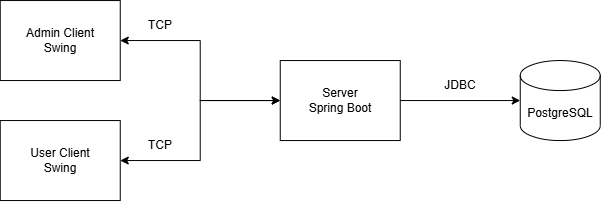
\includegraphics[width=\linewidth]{images/System Overview.drawio.png}
  \caption{Overall architecture of the chat system.}
  \label{fig:system-architecture}
\end{figure}

\begingroup
\small
\begin{longtable}{|L{3.1cm}|L{3.9cm}|L{\dimexpr\textwidth-7cm-6\tabcolsep-4\arrayrulewidth\relax}|}
  \caption{Technologies used in the system}
  \label{tab:technologies}\\
  \hline
  \textbf{Component} & \textbf{Technology} & \textbf{Purpose}\\
  \hline
  \endfirsthead
  \hline
  \textbf{Component} & \textbf{Technology} & \textbf{Purpose}\\
  \hline
  \endhead
  Programming language & Java 21 & Build the client applications and the backend\\
  \hline
  Windows interface & Java Swing & Build the administrator and user interfaces\\
  \hline
  Backend framework & Spring Boot & Organise the backend and the business logic\\
  \hline
  Client--server communication & TCP sockets &
  Exchange requests, responses and messages between clients and the server\\
  \hline
  Database & PostgreSQL & Store the system data\\
  \hline
  Data access & JDBC and the PostgreSQL JDBC Driver &
  Connect the backend to the database and run queries\\
  \hline
  Project management & Maven & Manage libraries, compile and package the applications\\
  \hline
  Testing & JUnit & Test the application components\\
  \hline
  Source control & Git and GitHub & Track changes and develop together\\
  \hline
\end{longtable}
\endgroup

In Version 1, the team focuses on the interface design of both subsystems and on
the database. The architecture above guides the implementation stage; the backend
and the socket communication do not have to be finished in this version.

\clearpage
\subsection{Component design}
\label{subsec:component-design}

This part defines the scope of the two client applications, the role of the
backend and the planned groups of data. The function lists are the reference for
checking the interface and the database design in V1; they are not a list of
finished functions. The screens, table structures and data relationships are
described in the matching detailed design parts.

\subsubsection{User application -- Java Swing}
\label{subsubsec:client-user}

The V1 user interface is built with Java Swing on Windows, for managing the
account, connecting with friends and exchanging messages. The subsystem of the
functions in this table is User. Function codes are independent of task codes and
of the order in which the report presents them.

\begingroup
\small
\begin{longtable}{|C{1.2cm}|L{\dimexpr\textwidth-1.2cm-4\tabcolsep-3\arrayrulewidth\relax}|}
  \caption{Functions of the user subsystem}
  \label{tab:user-features}\\
  \hline
  \textbf{Code} & \textbf{Function and scope}\\
  \hline
  \endfirsthead
  \hline
  \textbf{Code} & \textbf{Function and scope}\\
  \hline
  \endhead
  \hypertarget{F01}{\texttt{F01}} & \textbf{Register an account.}\\
  \hline
  \hypertarget{F02}{\texttt{F02}} & \textbf{Sign in.}\\
  \hline
  \hypertarget{F03}{\texttt{F03}} &
  \textbf{Update account information:} the profile editing interface, with the
  fields that match the user profile in \hyperlink{F13}{F13}.\\
  \hline
  \hypertarget{F04}{\texttt{F04}} &
  \textbf{Reset password:} generate a random password and send it by email.\\
  \hline
  \hypertarget{F05}{\texttt{F05}} & \textbf{Change password.}\\
  \hline
  \hypertarget{F06}{\texttt{F06}} &
  \textbf{Manage friends:} show the list, filter by name and see online/offline
  status; find people and send friend requests; unfriend; block and unfriend at once
  so the blocked person cannot send a request again.\\
  \hline
  \hypertarget{F07}{\texttt{F07}} &
  \textbf{Handle friend requests:} show, filter by name, accept or decline.\\
  \hline
  \hypertarget{F08}{\texttt{F08}} &
  \textbf{View online friends:} filter by name, start a chat or create a group.\\
  \hline
  \hypertarget{F09}{\texttt{F09}} &
  \textbf{Find people:} search by name or username, never showing people who
  blocked you; from the results, start a chat or create a group.\\
  \hline
  \hypertarget{F10}{\texttt{F10}} &
  \textbf{Report spam:} report an unwanted message received from someone.\\
  \hline
  \hypertarget{F11}{\texttt{F11}} &
  \textbf{Private chat and history:} real-time messaging when online; messages are
  kept for offline people to read later; view the history, delete all of it or some
  messages; search one or all conversations and jump to the result; call an LLM to
  rewrite or suggest messages.\\
  \hline
  \hypertarget{F12}{\texttt{F12}} &
  \textbf{Group chat:} create a group with at least one other username, rename it,
  add members, make members group admins, chat and encrypt the group; only group
  admins can remove members.\\
  \hline
\end{longtable}
\endgroup

In V1, this list is used to check the user screens against the requirements.
Sending messages, sending email, calling an LLM and group encryption do not have to
work yet at this stage; the preview only simulates their results with in-memory
sample data.

\paragraph{Navigation and screen list}
\label{par:user-navigation}
\mbox{}\par
When the V1 preview starts, the application opens the \textbf{Sign in} screen,
separate from \textbf{Admin Sign in}. From there the user can go to \textbf{Register}
or \textbf{Forgot password}. After signing in, the left sidebar is split into
\textbf{Messages} (\textbf{Chat}, \textbf{Group}), \textbf{People}
(\textbf{Friend}) and \textbf{Settings} (\textbf{Account}); the \textbf{Chat} screen
opens first. Each function lives on exactly one screen; other screens only link to
it. For example, the \textbf{Chat} button on the \textbf{Friend} page opens the
conversation on the \textbf{Chat} page, and the \textbf{Create group} button opens
the \textbf{Group} page's create form with the selected members.
Table~\ref{tab:user-screen-map} maps the Swing interface to the Figma prototype~\cite{ref:figma} and
to the function codes of the assignment. Labels in the table are quoted from the
interface.

\begingroup
\small
\begin{longtable}{|L{4.3cm}|L{\dimexpr\textwidth-4.3cm-4\tabcolsep-3\arrayrulewidth\relax}|}
  \caption{V1 user screens}
  \label{tab:user-screen-map}\\
  \hline
  \textbf{Screen} & \textbf{Functions and content}\\
  \hline
  \endfirsthead
  \hline
  \textbf{Screen} & \textbf{Functions and content}\\
  \hline
  \endhead
  \href{https://www.figma.com/design/maCogjZs9eOOhfkxsOZoIU?node-id=129-929}{Sign in}
  & \hyperlink{F02}{F02}. Username, password, the \textbf{Forgot password?} and
  \textbf{Create account} links. Error messages when a field is empty, when the
  username or password is wrong, and when an administrator has locked the account
  (\hyperlink{F13}{F13}).\\
  \hline
  \href{https://www.figma.com/design/maCogjZs9eOOhfkxsOZoIU?node-id=129-929}{Register}
  & \hyperlink{F01}{F01}. Username, full name, email, gender, date of birth and
  address (both optional), password and confirmation. Every invalid field is marked
  at once: username or email already used, invalid email or date of birth, password
  shorter than 8 characters or not matching. The new account is signed in right
  away.\\
  \hline
  \href{https://www.figma.com/design/maCogjZs9eOOhfkxsOZoIU?node-id=129-929}{Forgot password}
  & \hyperlink{F04}{F04}. Enter the account's email; the system generates a random
  password and sends it by email. V1 shows the email content inside the app; real
  email sending comes in V2.\\
  \hline
  \href{https://www.figma.com/design/maCogjZs9eOOhfkxsOZoIU?node-id=129-930}{Chat}
  & \hyperlink{F10}{F10}, \hyperlink{F11}{F11}, \hyperlink{F12}{F12} (group chat).
  One list for private and group conversations, with a name filter, an online dot
  and a lock icon for encrypted groups. My last message shows \textbf{Sent} when the
  server has it (group messages), \textbf{Waiting} when the recipient is offline and
  \textbf{Delivered} when the recipient has it: at once if they are online, or when
  they sign in again. The status is derived from \texttt{Message.deliveredAt}.
  Select one or more messages to \textbf{Delete for me} or \textbf{Report spam} (only
  one received message not reported yet, with a reason); \textbf{Clear history}
  clears the whole history for the current user only. \textbf{Search in chat} and
  \textbf{Search all messages} search one or all conversations and jump to the
  message. \textbf{Suggest} and \textbf{Improve} call the AI assistant to suggest or
  rewrite a message; both are refused in encrypted groups because the assistant may
  not read encrypted content. A chat with someone I blocked, someone who blocked me,
  or an account locked by an administrator (\hyperlink{F13}{F13}) shows a
  \textbf{Blocked} or \textbf{Locked} label and replaces the message box with an
  explanation.\\
  \hline
  \href{https://www.figma.com/design/maCogjZs9eOOhfkxsOZoIU?node-id=129-931}{Group}
  & \hyperlink{F12}{F12}. Group list with a name and role filter.
  \textbf{Create group} needs a group name and at least one other username.
  A group always has at least two people, so a member cannot be removed when only two
  are left. The group detail has \textbf{Rename}, \textbf{Add member},
  \textbf{Open chat} and the member table. \textbf{Make admin}, \textbf{Remove} and the
  \textbf{Encrypted group} toggle work only for group admins; for other members they
  are disabled with an explanation. A member whose account is locked carries the
  \textbf{Locked} label: a group admin can only \textbf{Remove} them, not
  \textbf{Make admin} them or add the account again. A removed member is recorded with
  \texttt{leftAt}, so their earlier messages stay in the history.\\
  \hline
  \href{https://www.figma.com/design/maCogjZs9eOOhfkxsOZoIU?node-id=129-932}{Friend}
  & \hyperlink{F06}{F06}--\hyperlink{F09}{F09}. \textbf{Friends} tab: name filter,
  online/offline status, \textbf{Chat}, \textbf{Unfriend}, \textbf{Block}.
  \textbf{Online} tab: online friends, select several people to create a group.
  \textbf{Requests} tab: accept or decline received requests, see sent requests.
  \textbf{Find people} tab: search by name or username, never showing people who
  blocked you; actions depend on the relationship (\textbf{Add friend},
  \textbf{Accept}, \textbf{Chat}, \textbf{Create group}, \textbf{Block}). A blocked
  person cannot send a friend request. A locked account carries the \textbf{Locked}
  label and accepts no actions: a locked friend only has \textbf{Unfriend}, a request
  from a locked account only has \textbf{Decline}, and \textbf{Find people} shows no
  buttons for it.\\
  \hline
  \href{https://www.figma.com/design/maCogjZs9eOOhfkxsOZoIU?node-id=129-933}{Account}
  & \hyperlink{F03}{F03}, \hyperlink{F05}{F05}. Profile card; \textbf{Edit profile}
  updates the full name, email, gender, date of birth and address; the username cannot
  be changed. \textbf{Change password} asks for the current password, the new password
  and its confirmation. \textbf{Sign Out} in the sidebar returns to the sign-in
  screen.\\
  \hline
\end{longtable}
\endgroup

\paragraph{V1 Java Swing screenshots}
\mbox{}\par
The screenshots below are captured from the Java Swing application in the
\texttt{user-client} module running on in-memory sample data. The signed-in sample
user is \textbf{Maya Chen}: sign in with the username \texttt{mayachen} and the
password \texttt{chatapp123}; every sample account shares this password, and
\texttt{linhng}, \texttt{owentran} and \texttt{ryanh} are locked. The sample data is
the same as in the administrator application. Changes last only for the preview
session. Real-time messaging, sending email, the AI assistant and group encryption
are simulated: the results look as designed, but there is no real server, email or
LLM yet.

\noindent\begin{minipage}{\linewidth}
  \centering
  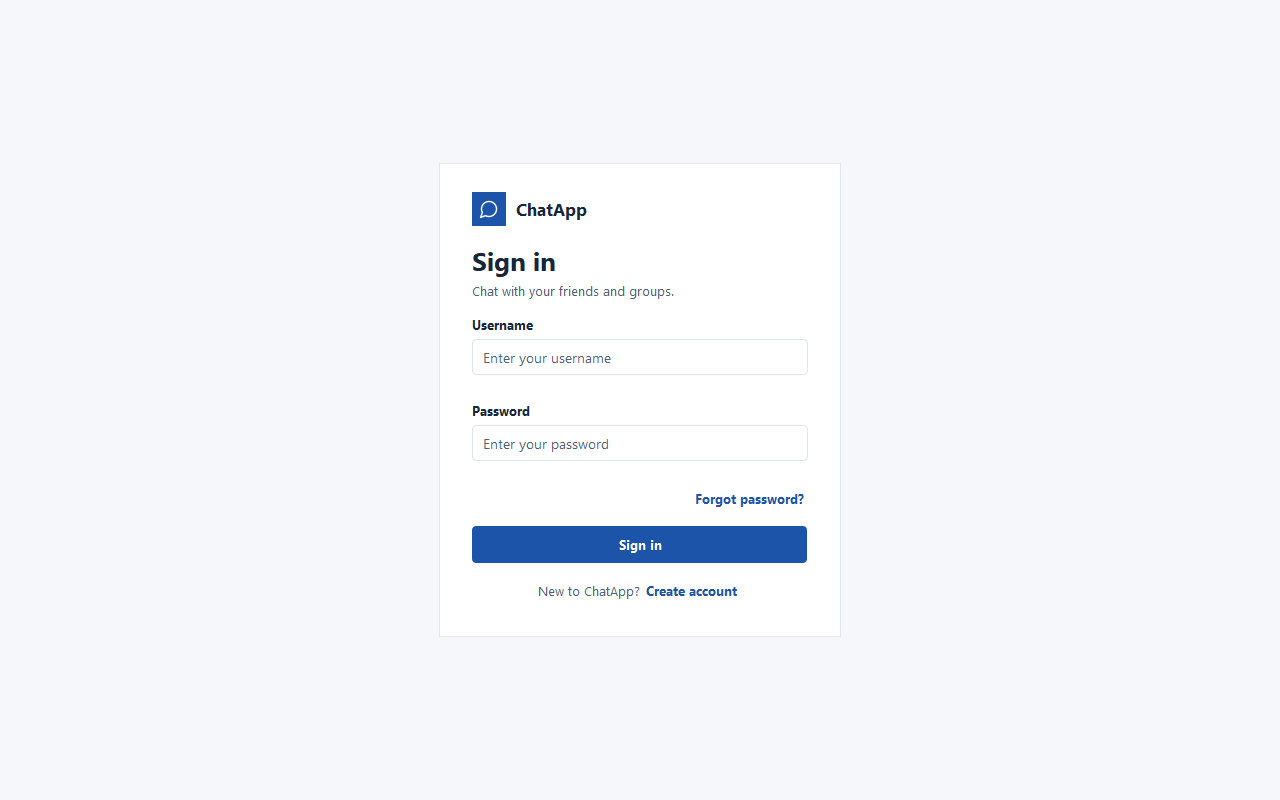
\includegraphics[width=.48\linewidth]{images/user-swing-login.png}\hfill
  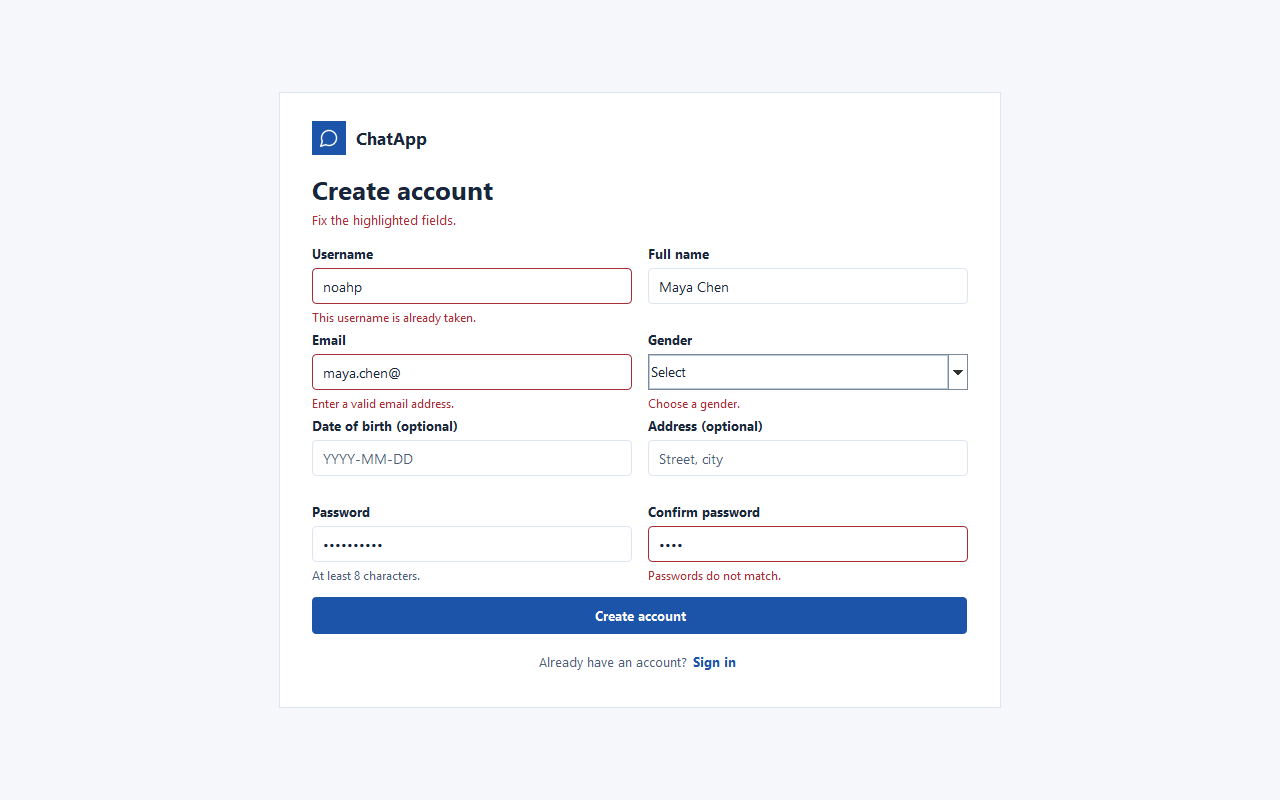
\includegraphics[width=.48\linewidth]{images/user-swing-register.png}
  \captionof{figure}{F02 and F01. Sign in and register, with input checks.}
  \label{fig:user-swing-login-register}
\end{minipage}

\noindent\begin{minipage}{\linewidth}
  \centering
  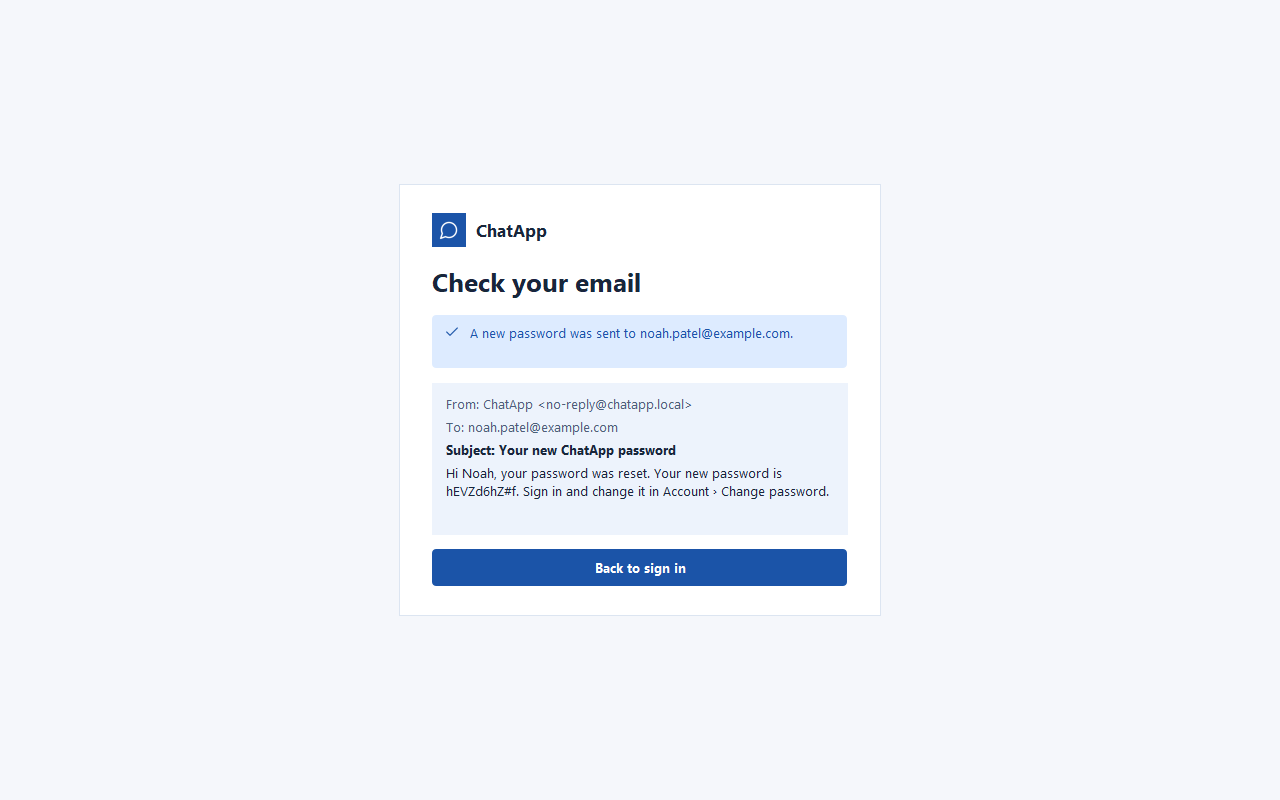
\includegraphics[width=.74\linewidth]{images/user-swing-forgot-password.png}
  \captionof{figure}{F04. The new random password and the email sent to the user.}
  \label{fig:user-swing-forgot-password}
\end{minipage}

\noindent\begin{minipage}{\linewidth}
  \centering
  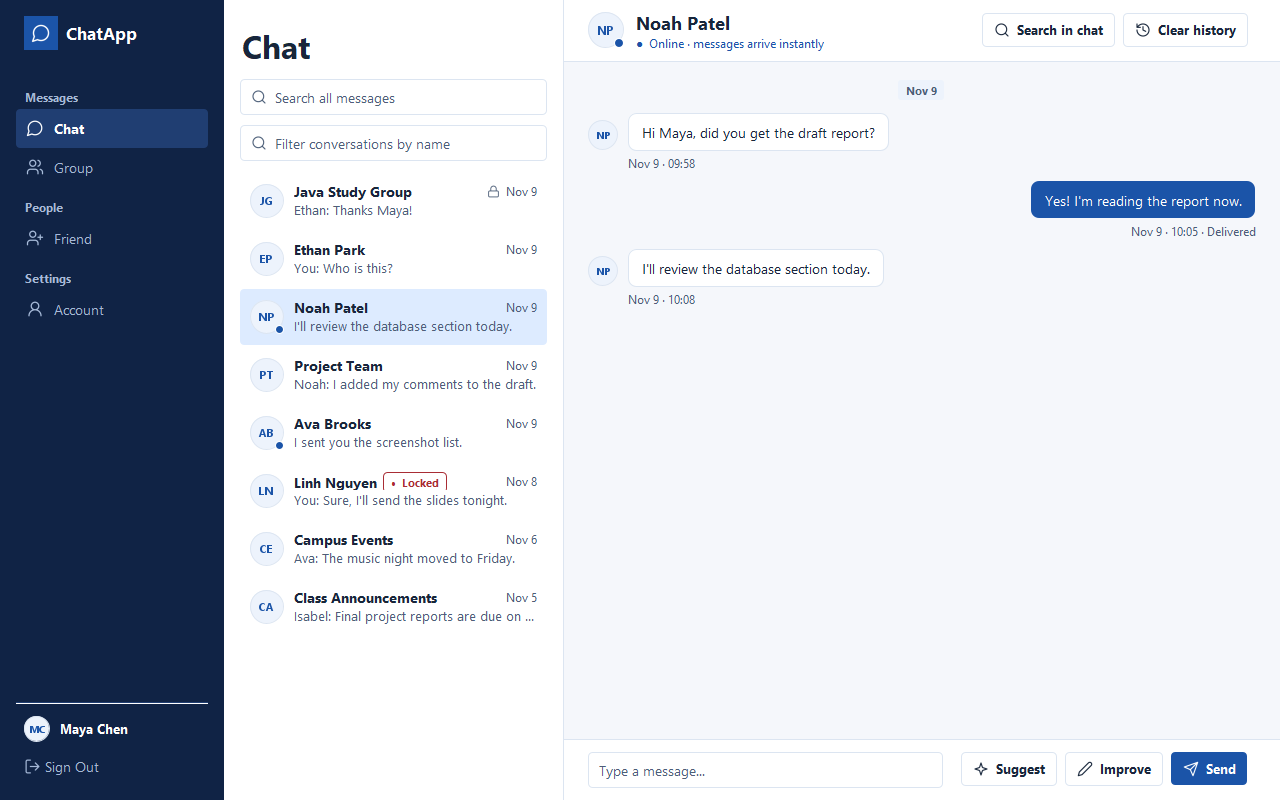
\includegraphics[width=.48\linewidth]{images/user-swing-chat.png}\hfill
  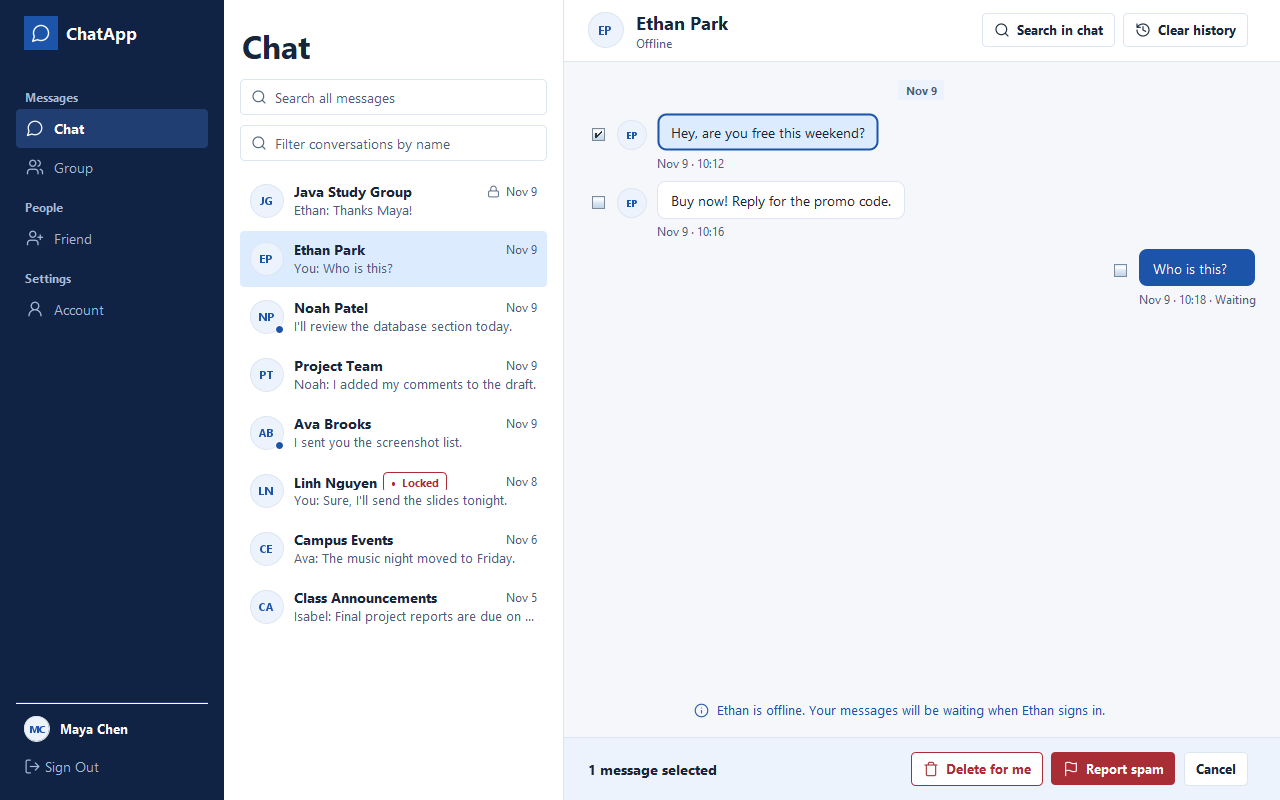
\includegraphics[width=.48\linewidth]{images/user-swing-chat-select.png}
  \captionof{figure}{F11 and F10. Chat with an online friend, message Delivered; select messages to delete for yourself or report spam; a message to an offline friend stays Waiting until that person signs in.}
  \label{fig:user-swing-chat}
\end{minipage}

\noindent\begin{minipage}{\linewidth}
  \centering
  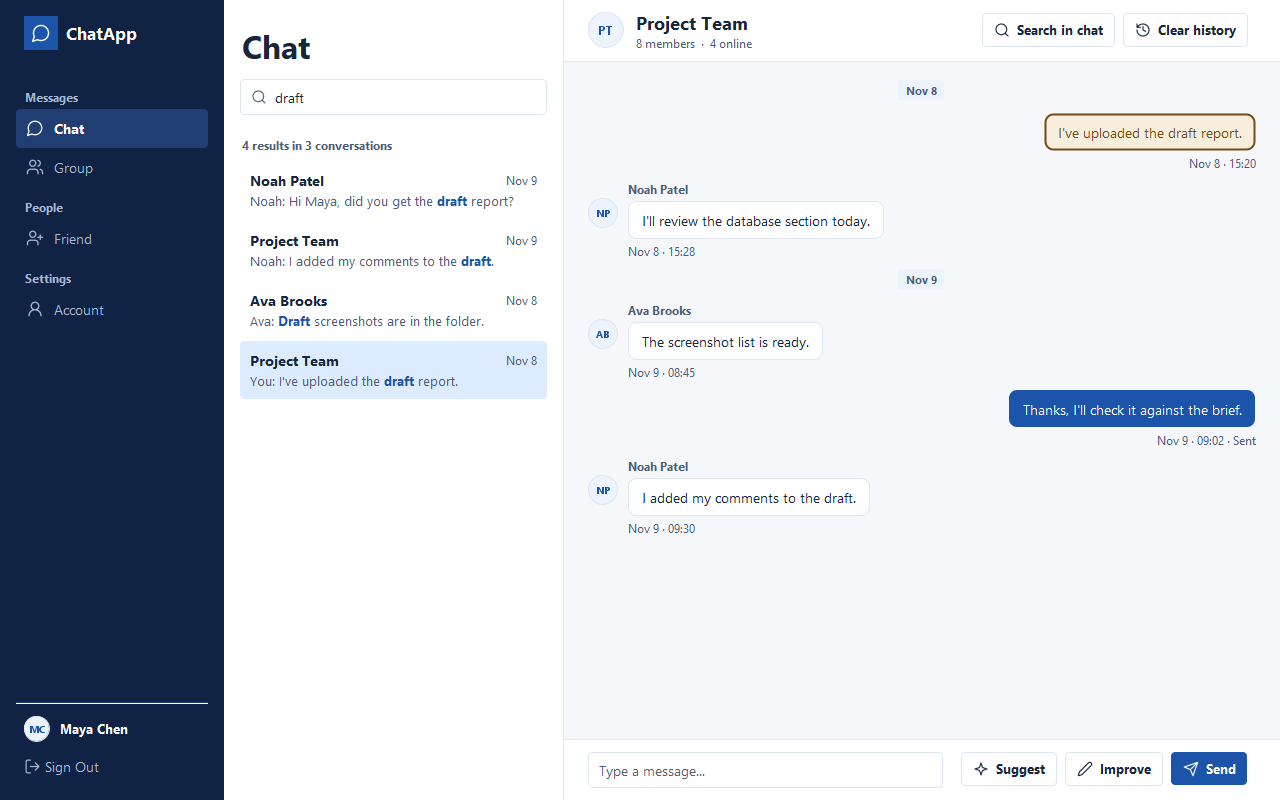
\includegraphics[width=.48\linewidth]{images/user-swing-chat-search.png}\hfill
  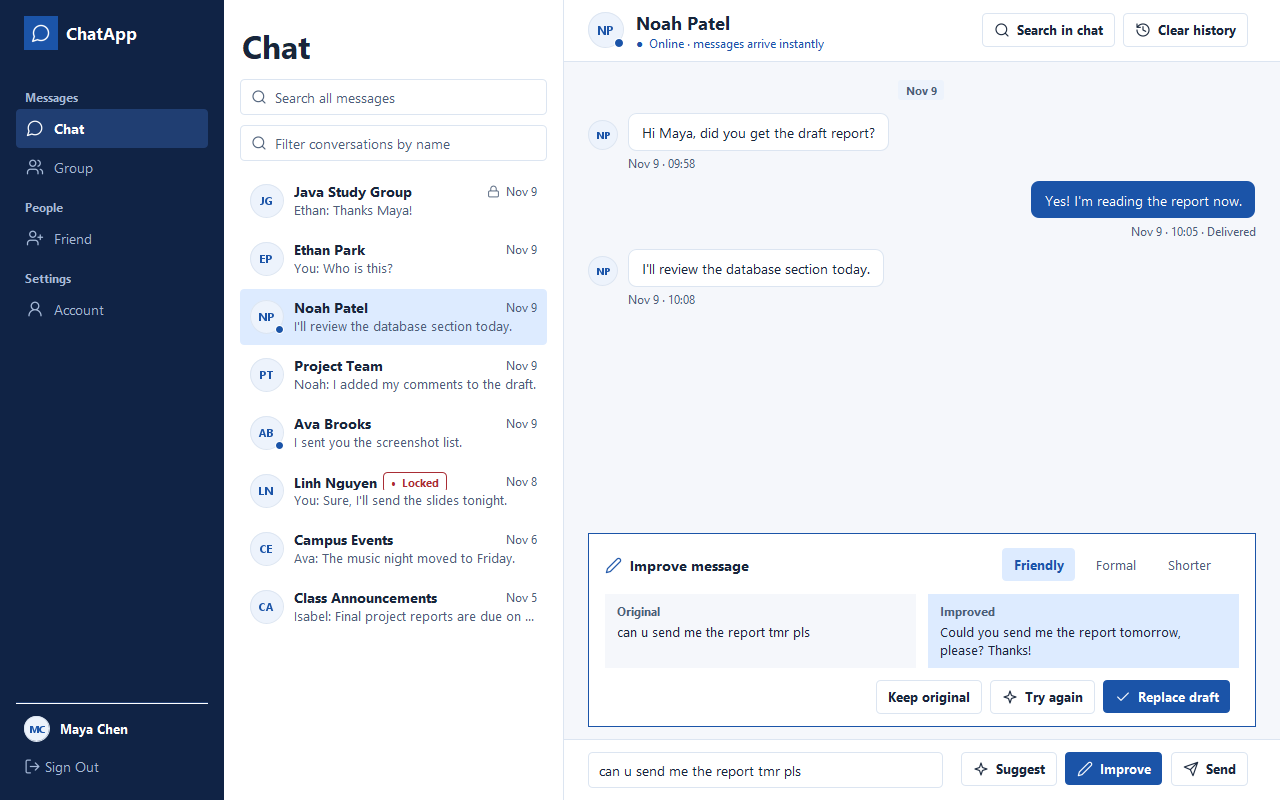
\includegraphics[width=.48\linewidth]{images/user-swing-chat-llm.png}
  \captionof{figure}{F11. Search all conversations and jump to the message; the AI assistant rewrites a message.}
  \label{fig:user-swing-chat-search-llm}
\end{minipage}

\noindent\begin{minipage}{\linewidth}
  \centering
  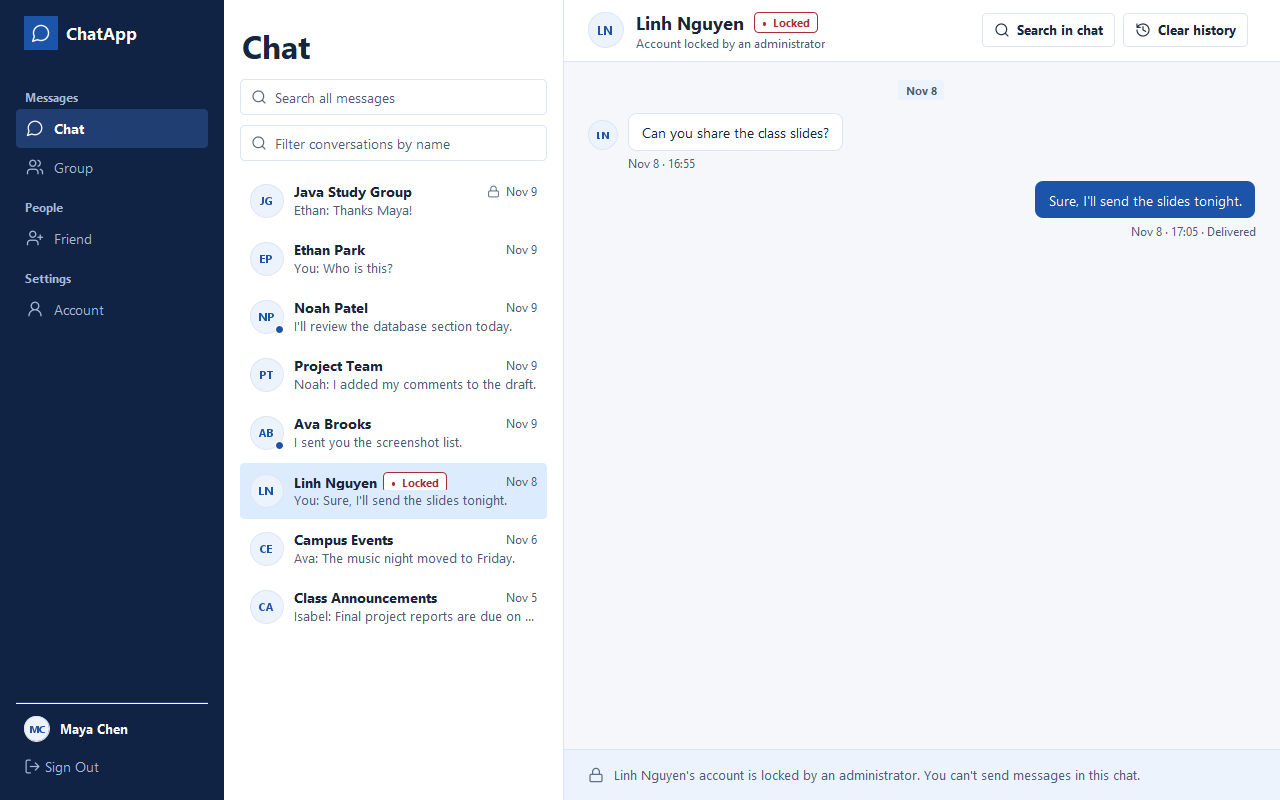
\includegraphics[width=.74\linewidth]{images/user-swing-chat-locked.png}
  \captionof{figure}{F11 and F13. A chat with an account locked by an administrator: Locked label, no sending.}
  \label{fig:user-swing-chat-locked}
\end{minipage}

\noindent\begin{minipage}{\linewidth}
  \centering
  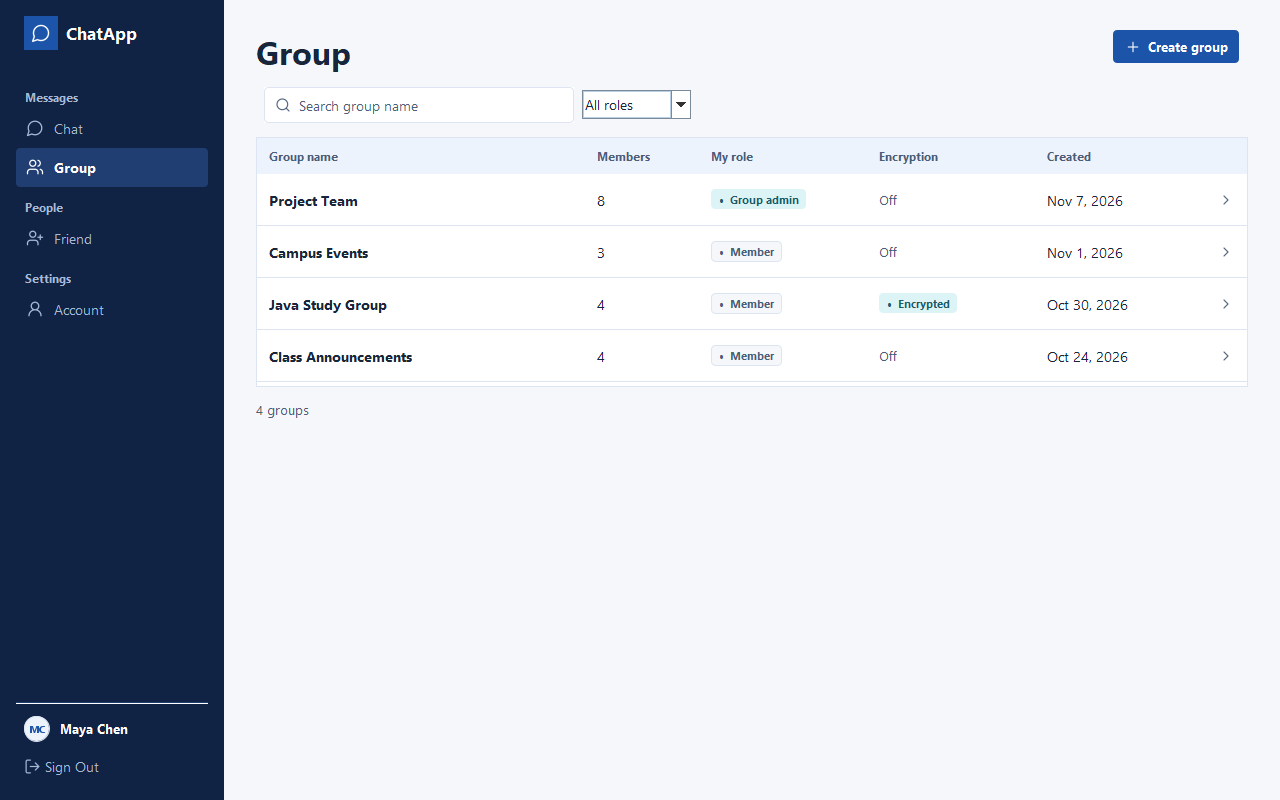
\includegraphics[width=.48\linewidth]{images/user-swing-group.png}\hfill
  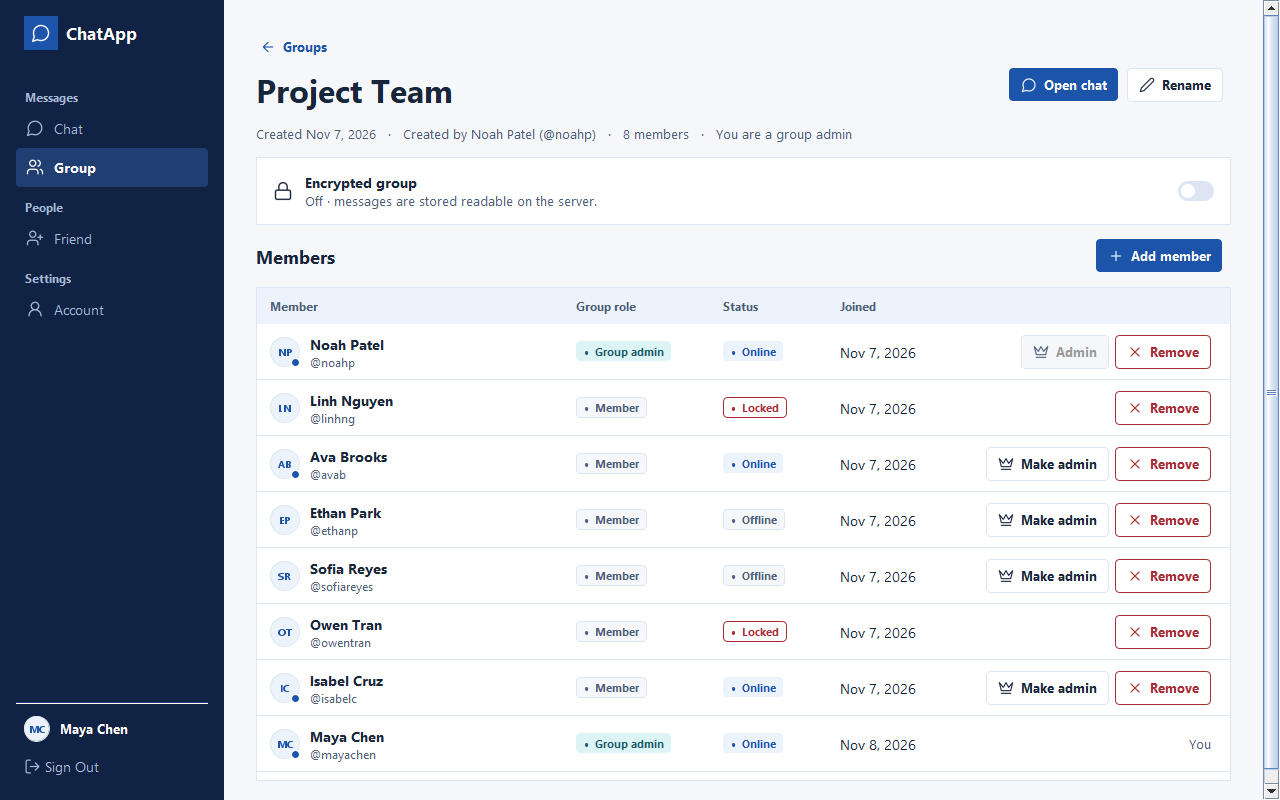
\includegraphics[width=.48\linewidth]{images/user-swing-group-detail.png}
  \captionof{figure}{F12. Group list and group detail with group admin rights; a locked member can only be removed.}
  \label{fig:user-swing-group}
\end{minipage}

\noindent\begin{minipage}{\linewidth}
  \centering
  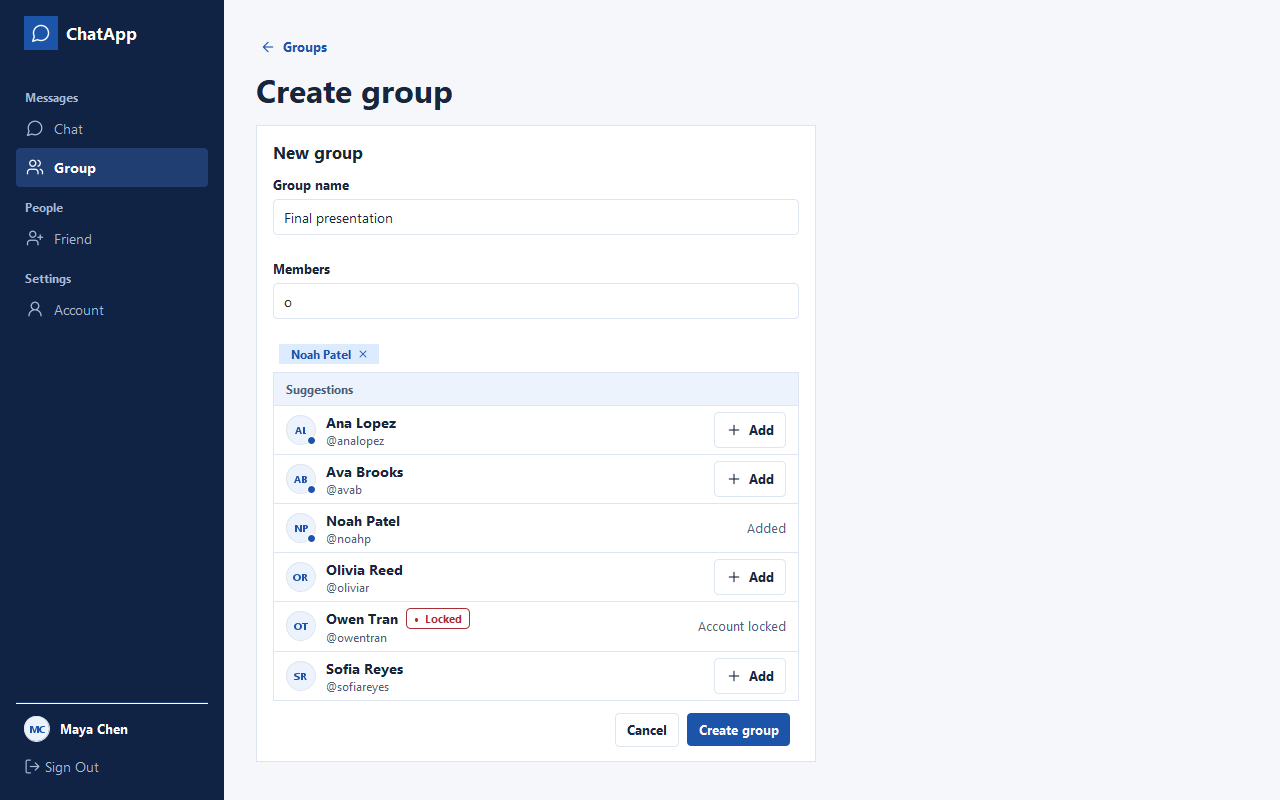
\includegraphics[width=.74\linewidth]{images/user-swing-group-create.png}
  \captionof{figure}{F12. Create a group with at least one other username.}
  \label{fig:user-swing-group-create}
\end{minipage}

\noindent\begin{minipage}{\linewidth}
  \centering
  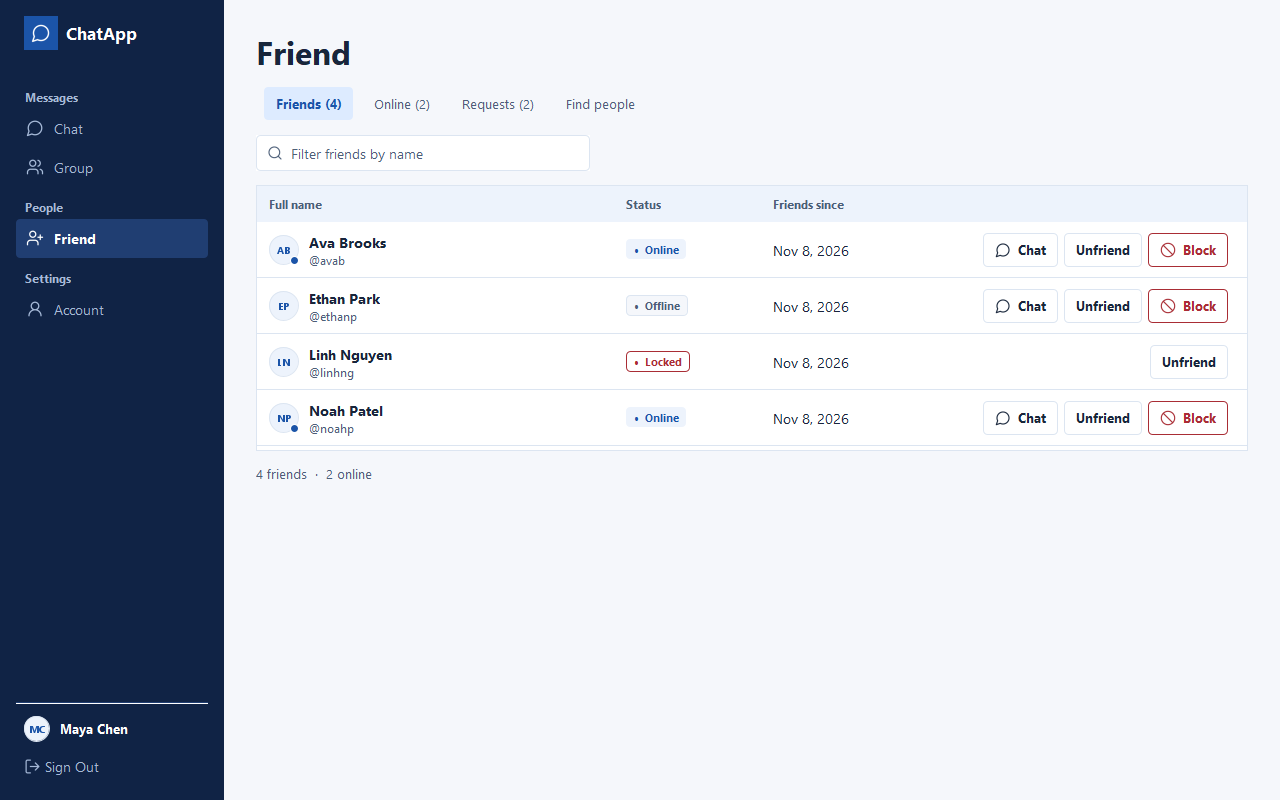
\includegraphics[width=.48\linewidth]{images/user-swing-friend.png}\hfill
  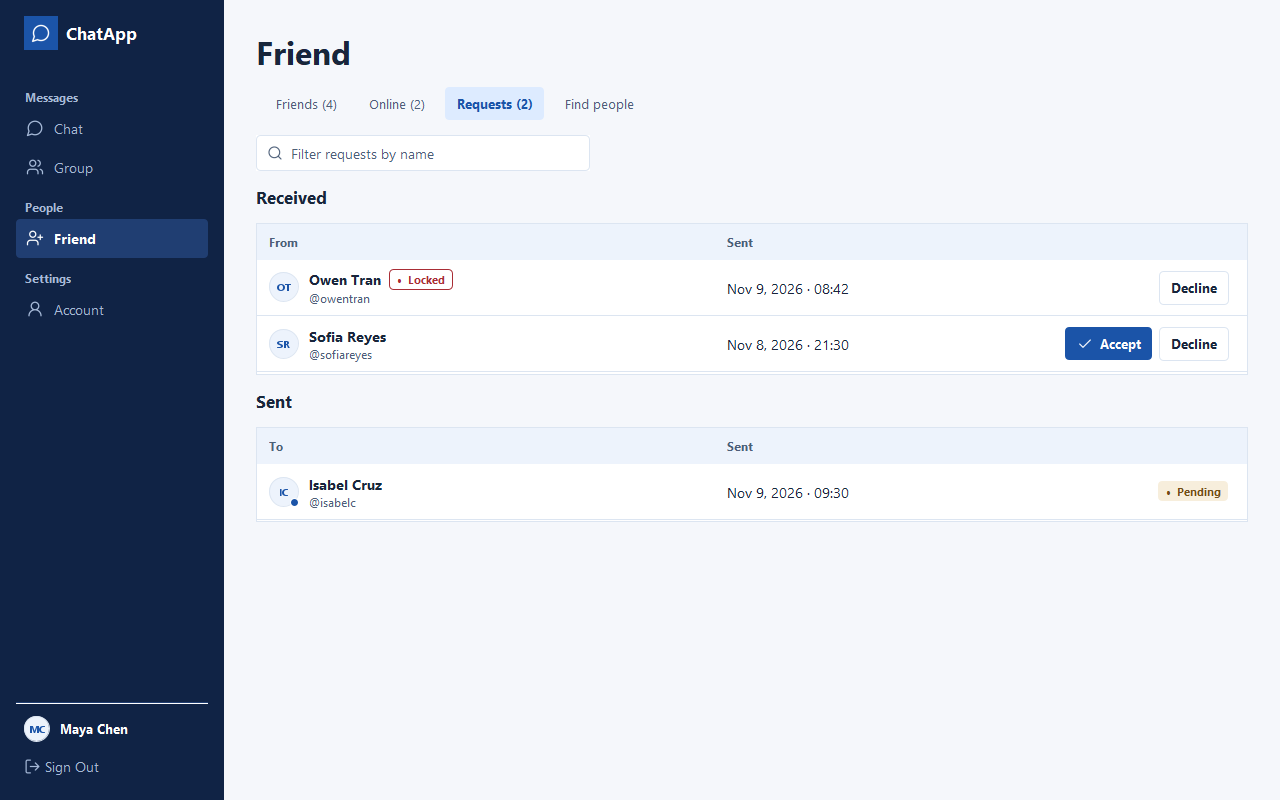
\includegraphics[width=.48\linewidth]{images/user-swing-friend-requests.png}
  \captionof{figure}{F06 and F07. Friend list and friend requests; locked accounts carry the Locked label.}
  \label{fig:user-swing-friend}
\end{minipage}

\noindent\begin{minipage}{\linewidth}
  \centering
  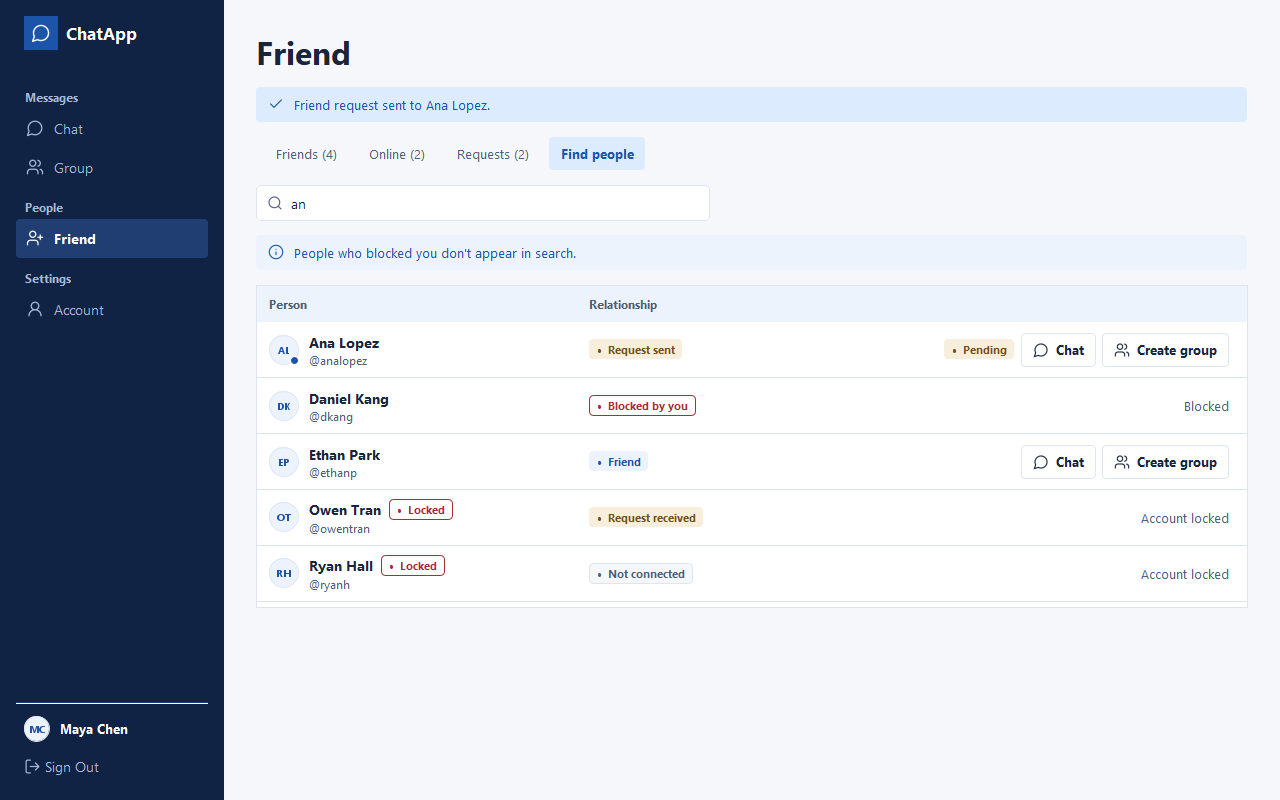
\includegraphics[width=.48\linewidth]{images/user-swing-find-people.png}\hfill
  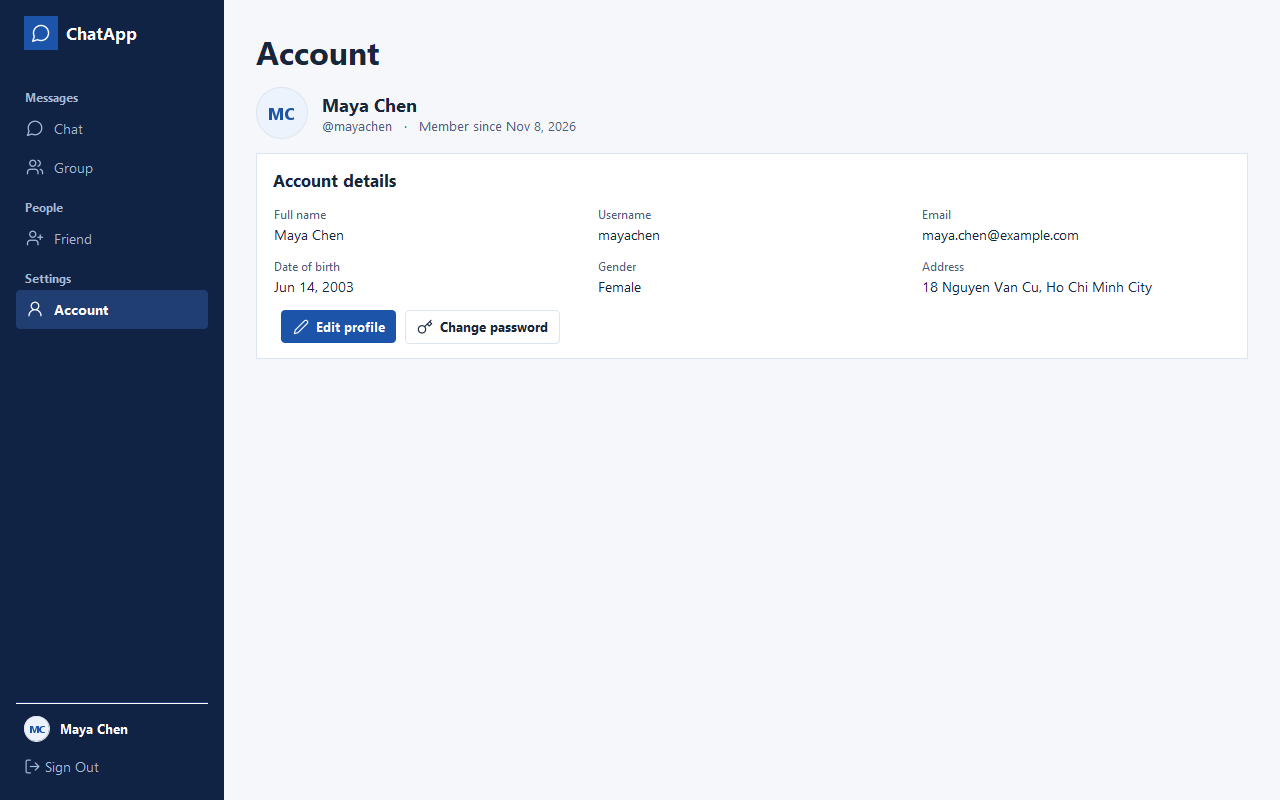
\includegraphics[width=.48\linewidth]{images/user-swing-account.png}
  \captionof{figure}{F09 and F03. Find people and send a friend request; the account profile.}
  \label{fig:user-swing-find-account}
\end{minipage}


\clearpage
\subsubsection{Administrator application -- Java Swing}
\label{subsubsec:client-admin}

The V1 administrator interface is built with Java Swing on Windows, for managing
and monitoring the system. The list below assigns the function codes used to map
functions to the tasks in Section~\ref{subsec:task-plan}.
The subsystem of the functions in this table is the system Admin, which is not the
same as the group admin role in a chat group.

\begingroup
\small
\begin{longtable}{|C{1.2cm}|L{\dimexpr\textwidth-1.2cm-4\tabcolsep-3\arrayrulewidth\relax}|}
  \caption{Functions of the administrator subsystem}
  \label{tab:admin-features}\\
  \hline
  \textbf{Code} & \textbf{Function and scope}\\
  \hline
  \endfirsthead
  \hline
  \textbf{Code} & \textbf{Function and scope}\\
  \hline
  \endhead
  \hypertarget{F13}{\texttt{F13}} &
  \textbf{Manage accounts:} view, add, update, delete; lock/unlock accounts;
  update passwords; view a user's sign-in history and friend list.
  User information includes the username, full name, address, date of birth,
  gender and email.
  Filter by name, username or status; sort by name or creation date.\\
  \hline
  \hypertarget{F14}{\texttt{F14}} &
  \textbf{View sign-ins:} show the time, username and full name,
  in time order.\\
  \hline
  \hypertarget{F15}{\texttt{F15}} &
  \textbf{View chat groups:} filter by name; sort by name or creation time;
  view the members and admins of each group.\\
  \hline
  \hypertarget{F16}{\texttt{F16}} &
  \textbf{View and handle spam reports:} filter by year and username;
  sort by time or username; lock the reported account.\\
  \hline
  \hypertarget{F17}{\texttt{F17}} &
  \textbf{View new registrations:} choose a year, filter by name,
  sort by name or creation time.\\
  \hline
  \hypertarget{F18}{\texttt{F18}} &
  \textbf{Registrations chart:} choose a year and show the number of new
  registrations per month; the horizontal axis is the month, the vertical axis
  the number of new registrations.\\
  \hline
  \hypertarget{F19}{\texttt{F19}} &
  \textbf{Friend statistics:} show the number of direct friends and the count
  including friends of friends; filter by name and by the number of direct friends
  equal to, less than or greater than an entered value; sort by name or creation time.\\
  \hline
  \hypertarget{F20}{\texttt{F20}} &
  \textbf{View active users:} choose a year; see the number of app opens and how
  many people and groups were chatted with; filter by name and by activity count
  equal to, less than or greater than an entered value;
  sort by name or creation time.\\
  \hline
  \hypertarget{F21}{\texttt{F21}} &
  \textbf{Active users chart:} choose a year and show the number of people who
  opened the app each month; the horizontal axis is the month, the vertical axis
  the number of people who opened the app.\\
  \hline
\end{longtable}
\endgroup

In V1, this list is used to check the administrator screens against the
requirements, including the matching action, filter and sort controls.

\paragraph{Navigation and screen list}
\label{par:admin-navigation}
\mbox{}\par
The left sidebar is split into \textbf{Manage Accounts},
\textbf{Monitor \& Moderate} and \textbf{Analyze Usage}. When the V1 preview starts,
the application opens the \textbf{Admin Sign in} screen; after signing in, the
\textbf{Users} screen is shown. Table~\ref{tab:admin-screen-map}
maps the Swing interface to the Figma prototype~\cite{ref:figma} and to the
function codes of the assignment. Labels in the table are quoted from the interface.

\begingroup
\small
\begin{longtable}{|L{4.3cm}|L{\dimexpr\textwidth-4.3cm-4\tabcolsep-3\arrayrulewidth\relax}|}
  \caption{V1 administrator screens}
  \label{tab:admin-screen-map}\\
  \hline
  \textbf{Screen} & \textbf{Functions and content}\\
  \hline
  \endfirsthead
  \hline
  \textbf{Screen} & \textbf{Functions and content}\\
  \hline
  \endhead
  Admin Sign in
  & The administrator application's own sign-in screen, separate from the sign-in
  screen of the user application. It has a username, a password and a message when
  a field is empty. In V2 the server checks the password and the \texttt{ADMIN} role
  before opening a session; \textbf{Sign Out} returns to this screen.\\
  \hline
  \href{https://www.figma.com/design/maCogjZs9eOOhfkxsOZoIU?node-id=2-80}{Users}
  & \hyperlink{F13}{F13}. Account list and profile, add/edit form,
  password change, lock/unlock and delete confirmation. The profile has the
  \textbf{Login History} and \textbf{Friends \& Groups} tabs. The address and date of
  birth are optional. The account status is \textbf{Active} or \textbf{Locked};
  a locked account stays locked until an administrator unlocks it.\\
  \hline
  \href{https://www.figma.com/design/maCogjZs9eOOhfkxsOZoIU?node-id=16-822}{Account History}
  & \hyperlink{F14}{F14}, \hyperlink{F17}{F17}. \textbf{Sign-ins} shows the time,
  username and full name across the whole system. \textbf{New Accounts}
  shows the accounts created in the selected year, with search, sorting and a monthly
  registrations chart.\\
  \hline
  \href{https://www.figma.com/design/maCogjZs9eOOhfkxsOZoIU?node-id=25-1020}{Chat Groups}
  & \hyperlink{F15}{F15}. Group list with search and sorting. The group detail
  shows the creator, the creation time, the members and the group admins.
  \textbf{Activity} and \textbf{Monitoring} illustrate an extension for monitoring
  groups. The monthly chart counts activity, messages or members joining.\\
  \hline
  \href{https://www.figma.com/design/maCogjZs9eOOhfkxsOZoIU?node-id=38-1461}{Spam Reports}
  & \hyperlink{F16}{F16}. \textbf{Reports} lists the individual reports.
  \textbf{By account} groups them by account, with a status filter and the report
  history. The lock count and the lock/unlock log use the same selected year.
  The report detail shows the reporter, the reported account, the reason and the
  related message before the account lock is confirmed.\\
  \hline
  \href{https://www.figma.com/design/maCogjZs9eOOhfkxsOZoIU?node-id=53-934}{Analytics / Overview}
  & \hyperlink{F18}{F18}, \hyperlink{F21}{F21}. \textbf{Graph} selects the monthly
  chart for the year. \textbf{Registrations} counts created accounts;
  \textbf{Active users} counts distinct accounts that opened the app. The
  \textbf{Sign-ins} and \textbf{Messages sent} charts add more views of usage.\\
  \hline
  \href{https://www.figma.com/design/maCogjZs9eOOhfkxsOZoIU?node-id=53-1087}{Analytics / Friend Counts}
  & \hyperlink{F19}{F19}. The table shows the number of direct friends and the total
  number of people in the friend network. An account's detail has three collapsible
  lists: friends, chat groups, and friends of friends with their mutual friends.\\
  \hline
  \href{https://www.figma.com/design/maCogjZs9eOOhfkxsOZoIU?node-id=53-1279}{Analytics / Activity}
  & \hyperlink{F20}{F20}. The table for the selected year shows sign-ins, app opens,
  and the number of people and groups chatted with, each separately. By default
  \textbf{Any count} also shows accounts that opened the app without signing in
  again in the selected year. The \textbf{Monthly sign-ins} chart counts system-wide
  sign-ins in each month of that year. The \textbf{Active users} chart on
  \textbf{Overview} counts distinct accounts that opened the app.\\
  \hline
\end{longtable}
\endgroup

\paragraph{Period picker}
\mbox{}\par
The team applies the ``time period'' of the assignment (new registrations, active
users and filtering spam reports by time) as a calendar year, in line with the
yearly charts.
The \textbf{Period} button selects one calendar year shared by every administrator
screen that has a time filter. The selected year is kept when switching screens.
Time-based lists show the records from 1 January to 31 December of that year.
Every chart shows all 12 months from January to December, even when some months or
the whole year have no records.

\paragraph{V1 Java Swing screenshots}
\mbox{}\par
The screenshots below are rendered from the Java Swing application in the
\texttt{admin-client} module. The V1 build opens the \textbf{Admin Sign in} screen,
then the \textbf{Users} screen, and uses in-memory sample data. In V1 the sign-in
screen accepts any non-empty username and password (for example
\texttt{admin} / \texttt{admin}); the server checks the \texttt{ADMIN} role in V2. The
sample data is the same as in the user application. The administrator's display
name is \textbf{Admin}. Account changes last only for the preview session. The
password change form shows the input checks.

\noindent\begin{minipage}{\linewidth}
  \centering
  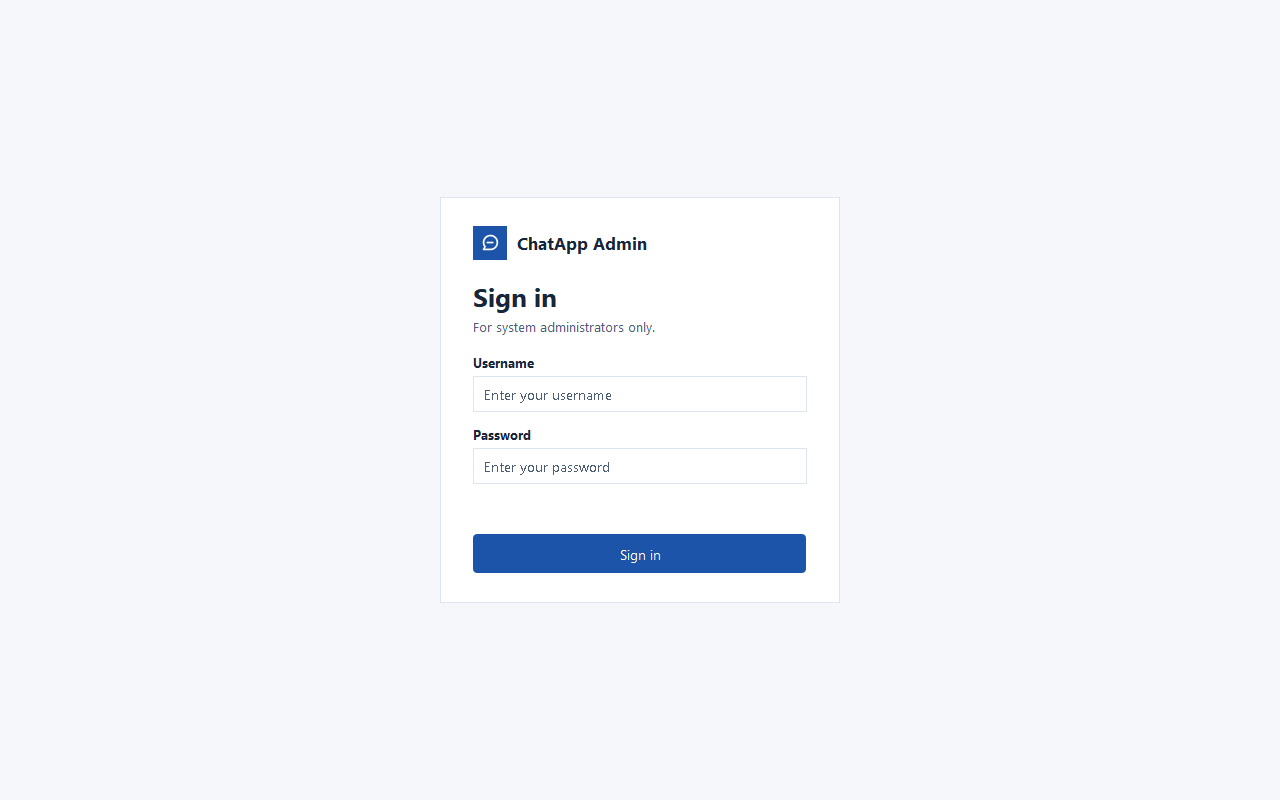
\includegraphics[width=.74\linewidth]{images/admin-swing-login.png}
  \captionof{figure}{Sign-in screen of the administrator application.}
  \label{fig:admin-swing-login}
\end{minipage}

\noindent\begin{minipage}{\linewidth}
  \centering
  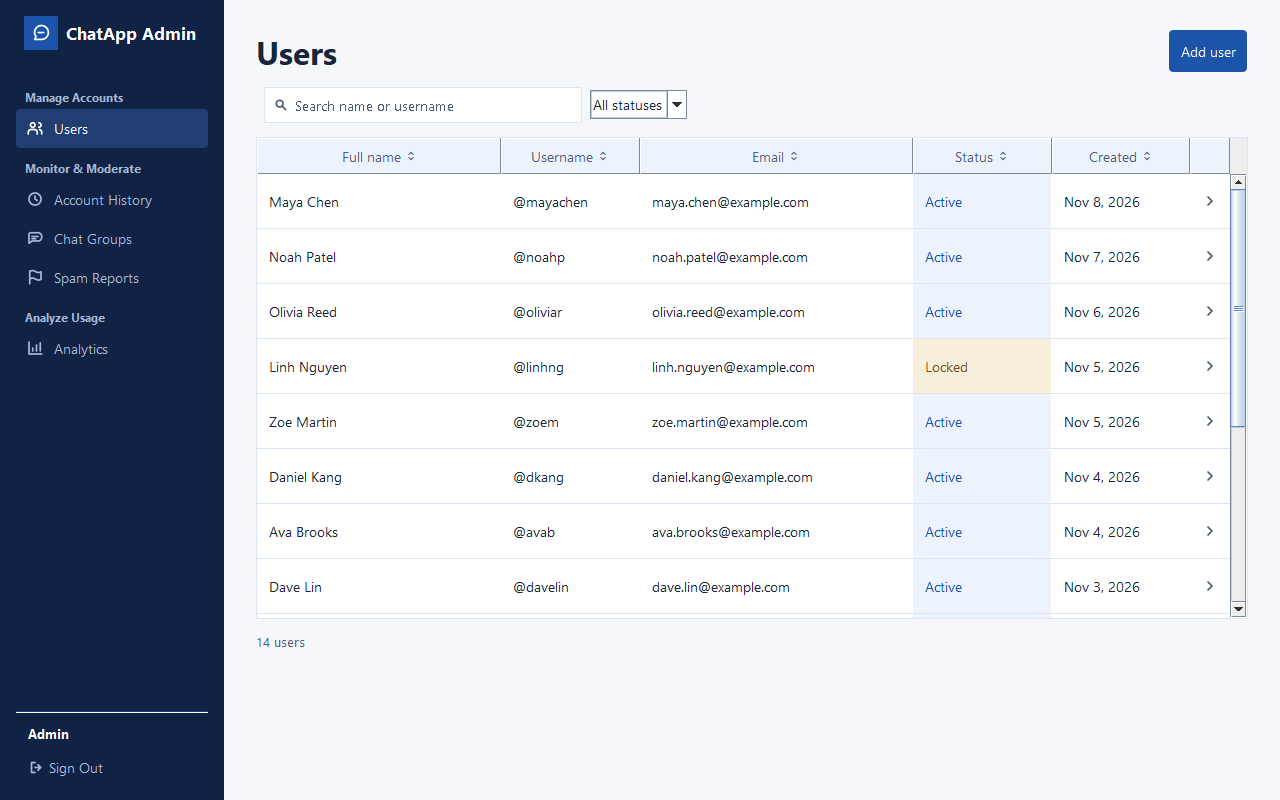
\includegraphics[width=.48\linewidth]{images/admin-swing-users.png}\hfill
  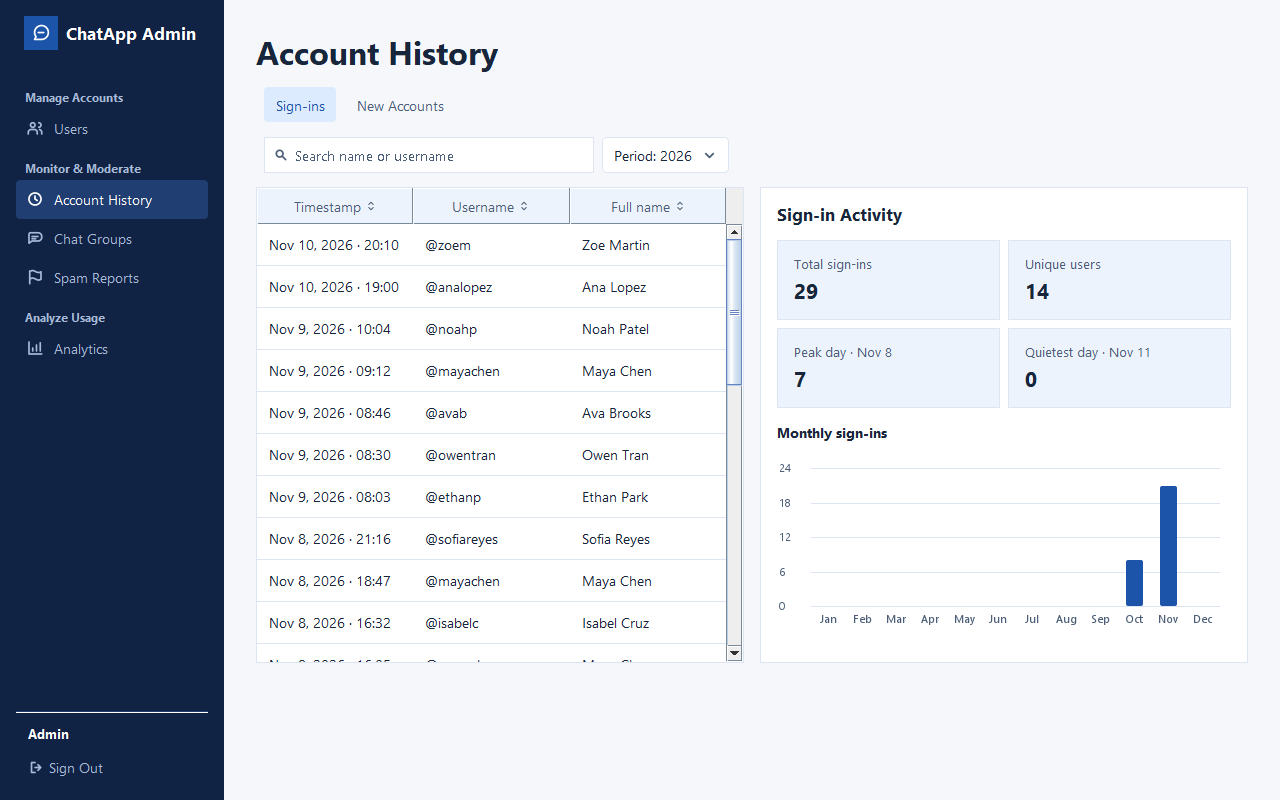
\includegraphics[width=.48\linewidth]{images/admin-swing-account-history.png}
  \captionof{figure}{F13 and F14. Account list and system-wide sign-in history.}
  \label{fig:admin-swing-users-history}
\end{minipage}

\noindent\begin{minipage}{\linewidth}
  \centering
  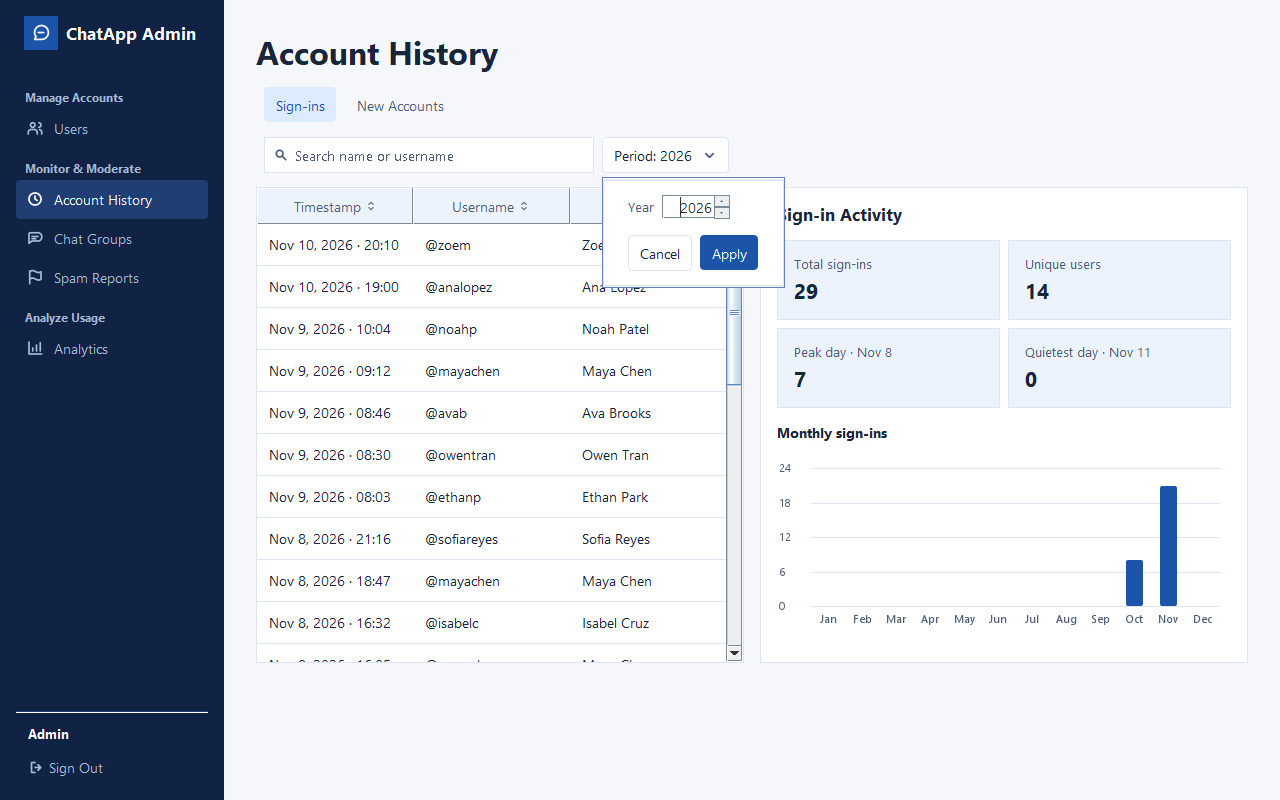
\includegraphics[width=.92\linewidth]{images/admin-swing-period-picker.png}
  \captionof{figure}{The shared year picker, opened from the Account History screen.}
  \label{fig:admin-swing-period}
\end{minipage}

\noindent\begin{minipage}{\linewidth}
  \centering
  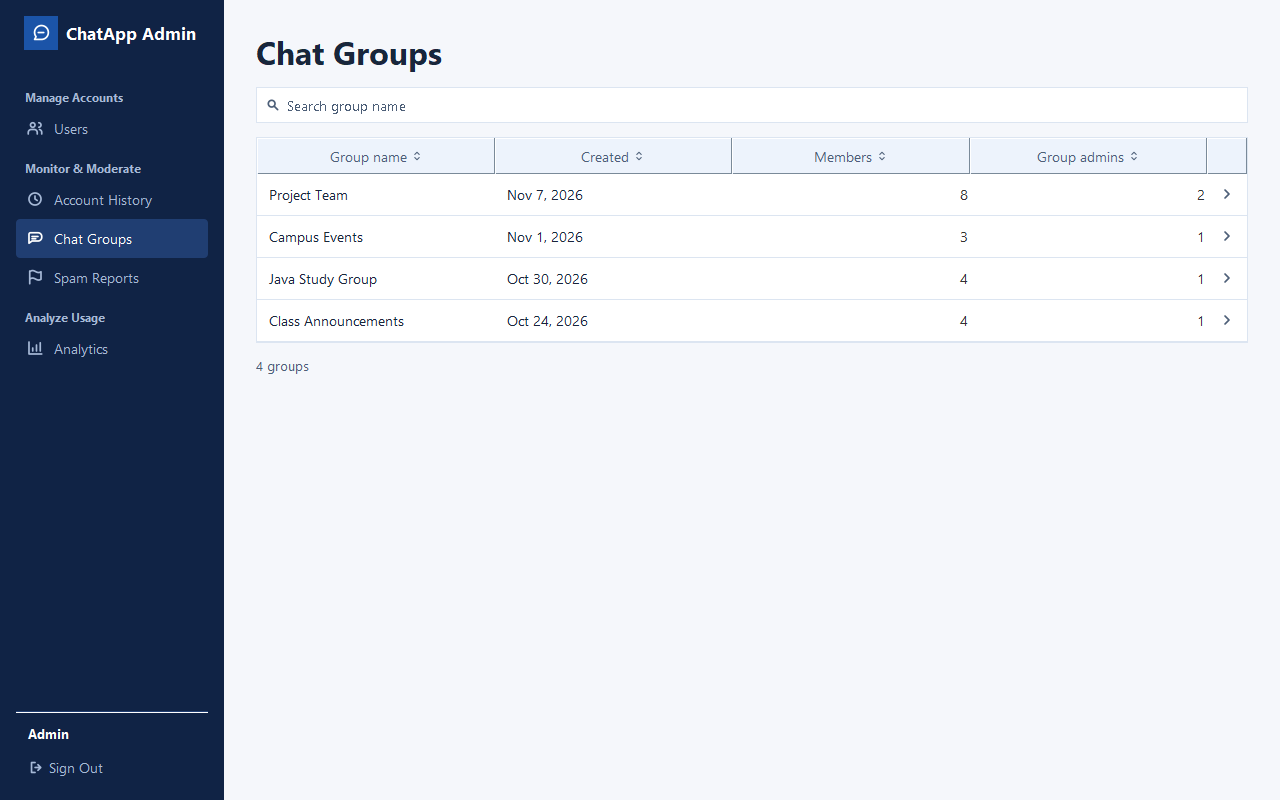
\includegraphics[width=.48\linewidth]{images/admin-swing-groups.png}\hfill
  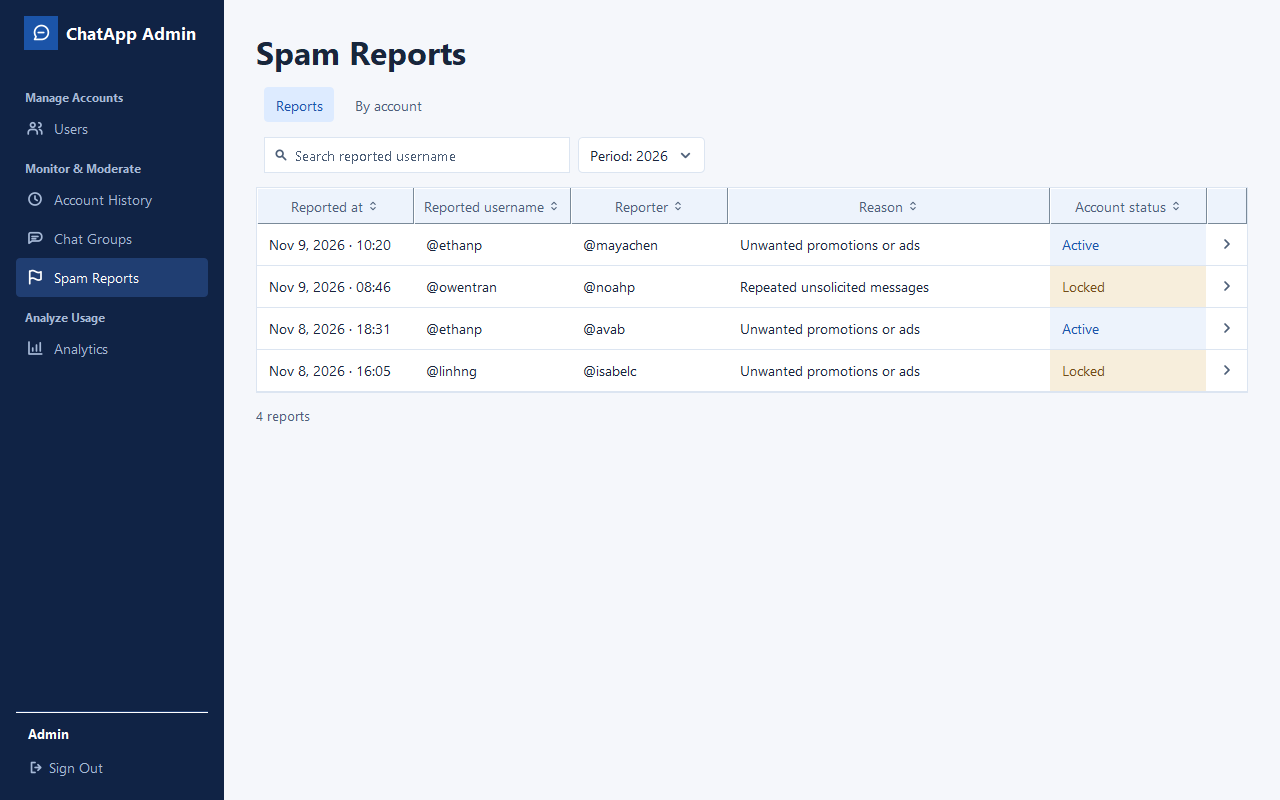
\includegraphics[width=.48\linewidth]{images/admin-swing-spam-reports.png}
  \captionof{figure}{F15 and F16. Chat groups and spam reports.}
  \label{fig:admin-swing-moderation}
\end{minipage}

\noindent\begin{minipage}{\linewidth}
  \centering
  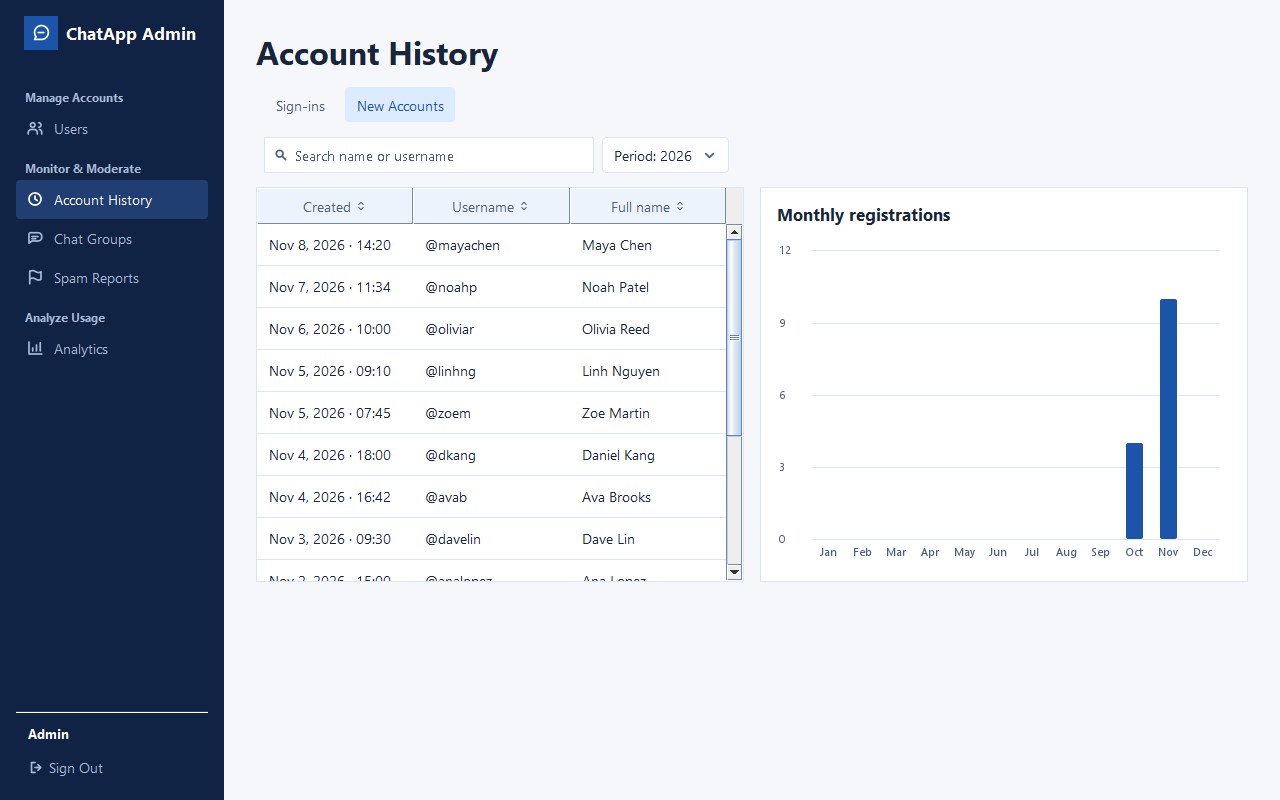
\includegraphics[width=.48\linewidth]{images/admin-swing-new-accounts.png}\hfill
  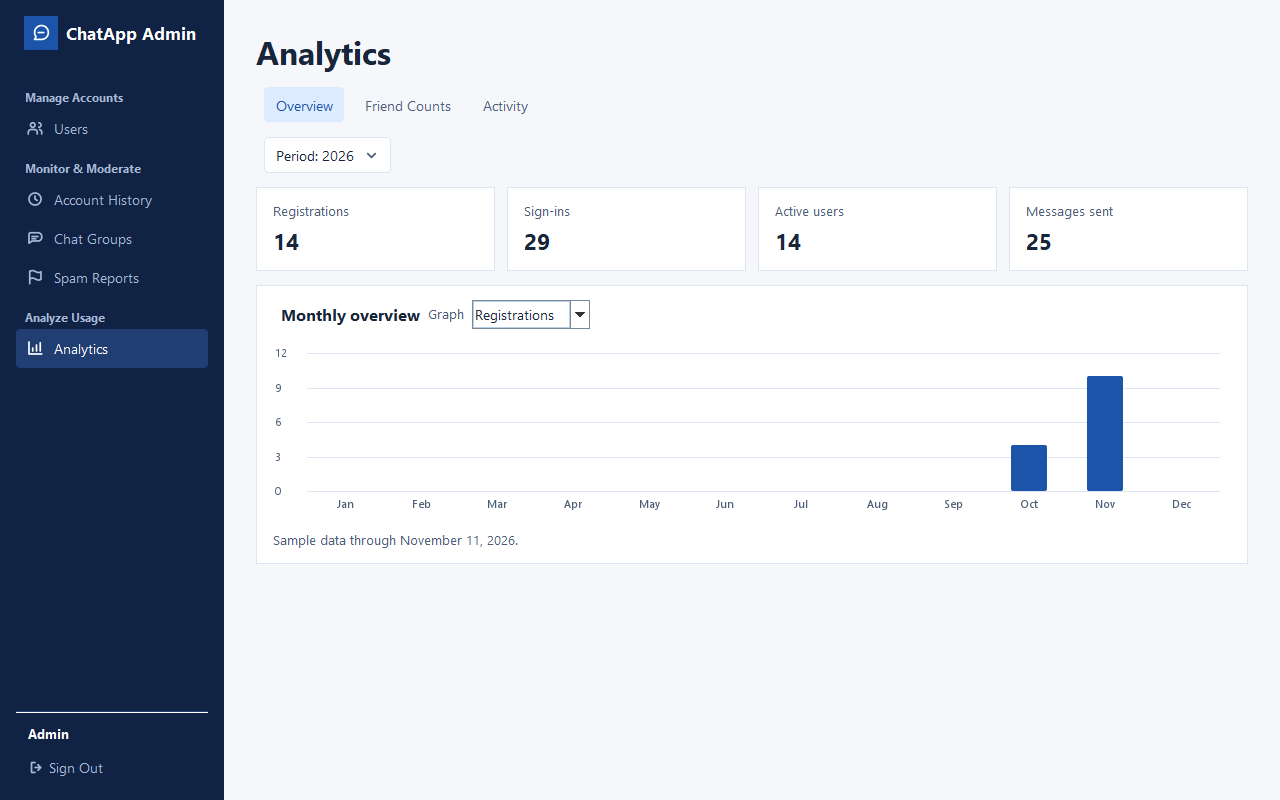
\includegraphics[width=.48\linewidth]{images/admin-swing-overview.png}
  \captionof{figure}{F17 and F18. New accounts in the selected year and the monthly registrations chart.}
  \label{fig:admin-swing-registrations}
\end{minipage}

\noindent\begin{minipage}{\linewidth}
  \centering
  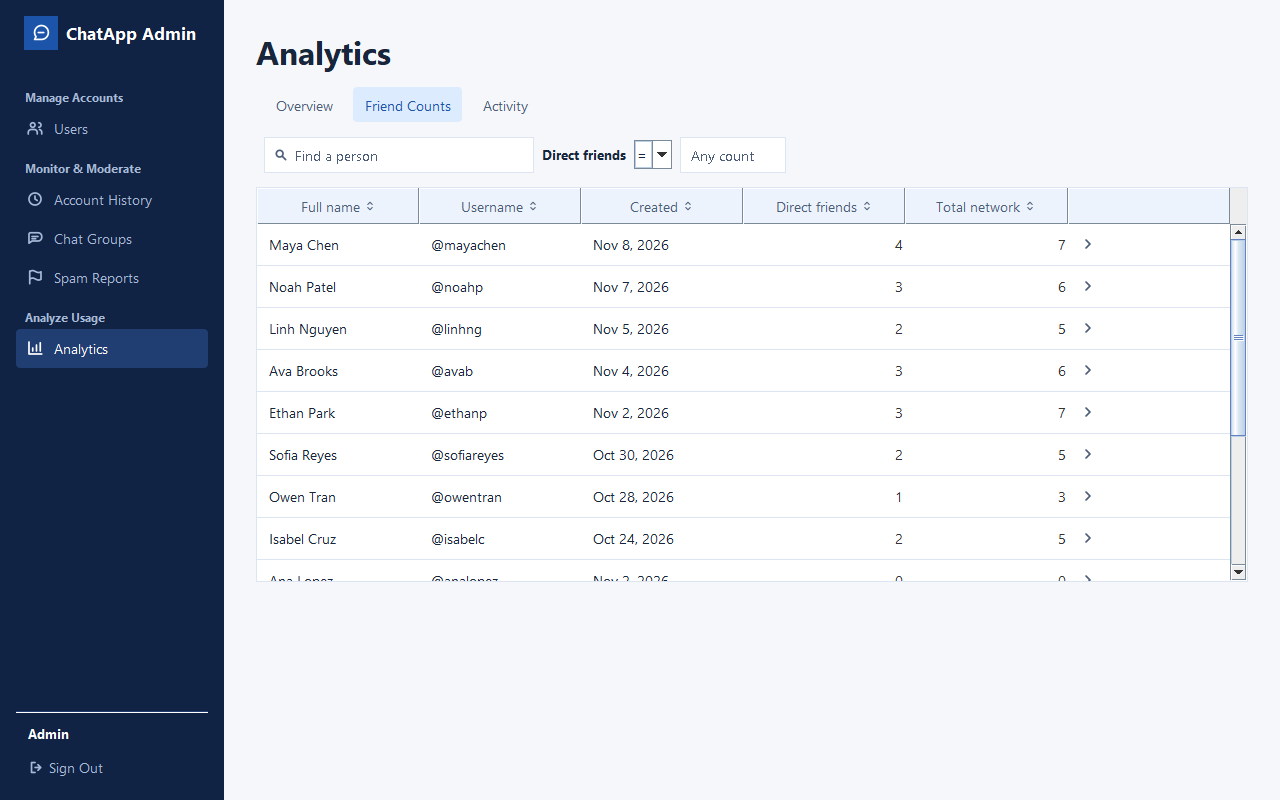
\includegraphics[width=.48\linewidth]{images/admin-swing-friend-counts.png}\hfill
  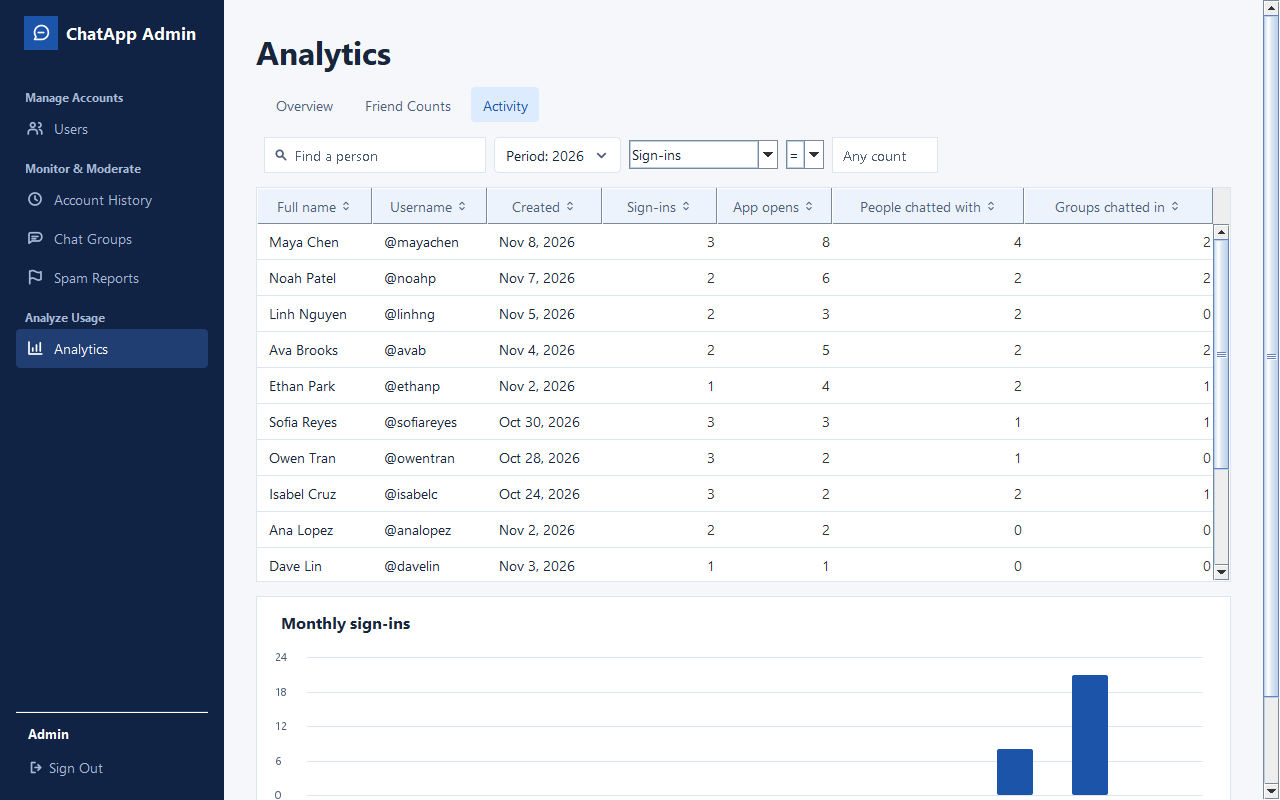
\includegraphics[width=.48\linewidth]{images/admin-swing-activity.png}
  \captionof{figure}{F19 and F20. Friend statistics and activity per account.}
  \label{fig:admin-swing-friends-activity}
\end{minipage}

\noindent\begin{minipage}{\linewidth}
  \centering
  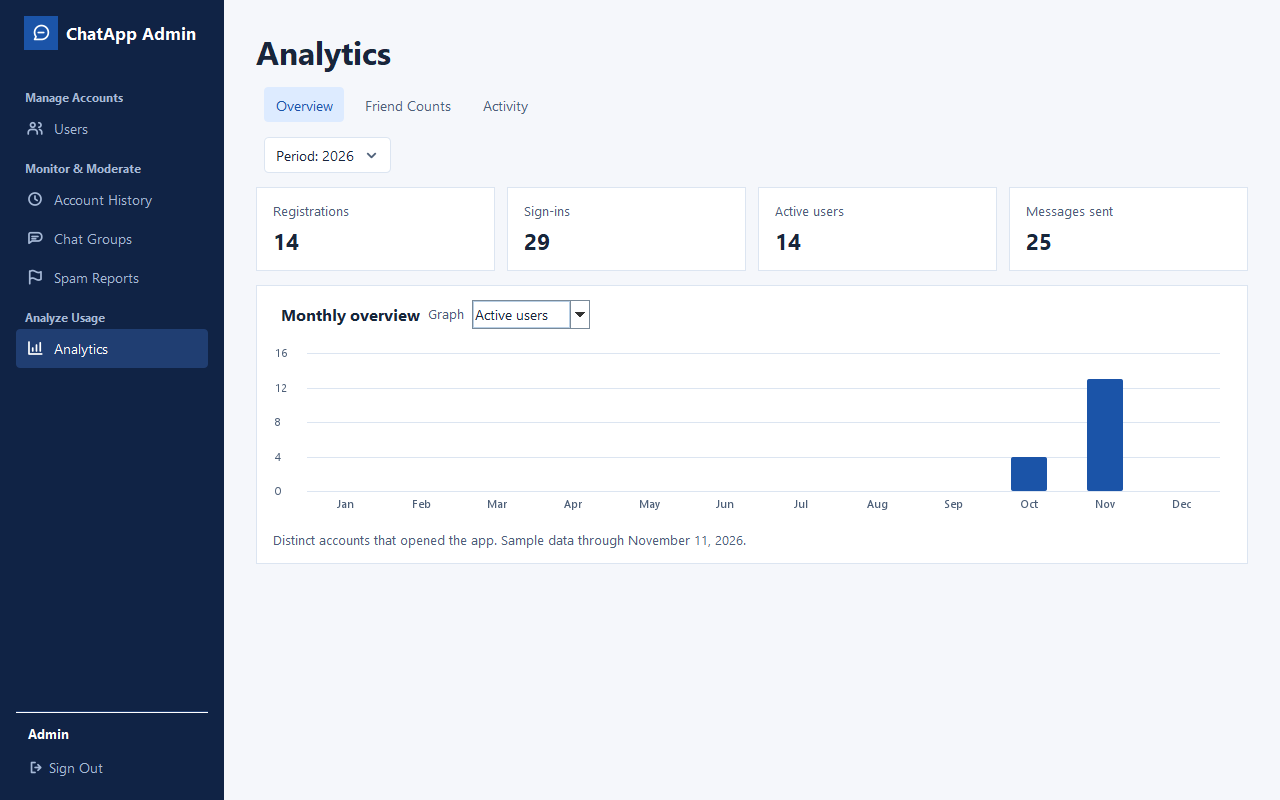
\includegraphics[width=.74\linewidth]{images/admin-swing-active-users.png}
  \captionof{figure}{F21. Distinct accounts that opened the app in each month.}
  \label{fig:admin-swing-active-users}
\end{minipage}


\clearpage
\subsubsection{Backend -- Spring Boot}
\label{subsubsec:backend-spring-boot}

The team chose Spring Boot to build the backend of the chat system. Spring Boot
supports building Spring applications through auto-configuration and management
of the application's components, which reduces the manual configuration needed
to start a project.

In this project, Spring Boot is planned to be used as follows:

\begingroup
\small
\begin{longtable}{|L{4.6cm}|L{\dimexpr\textwidth-4.6cm-4\tabcolsep-3\arrayrulewidth\relax}|}
  \caption{How Spring Boot is applied in the project}
  \label{tab:spring-boot-usage}\\
  \hline
  \textbf{Feature} & \textbf{How it is applied}\\
  \hline
  \endfirsthead
  \hline
  \textbf{Feature} & \textbf{How it is applied}\\
  \hline
  \endhead
  Component management and Dependency Injection &
  Manages the business logic, data access and server components, and
  provides them where they are needed\\
  \hline
  Auto-configuration &
  Configures components based on the libraries and settings declared
  in the project\\
  \hline
  External configuration &
  Declares the TCP port and the PostgreSQL connection settings in a configuration
  file instead of hard-coding them in the source code\\
  \hline
  Code organisation &
  Works with the split into services (business logic) and DAOs
  (Data Access Objects, the data access layer) to keep business logic
  apart from data queries\\
  \hline
  Packaging &
  Packages the backend as a stand-alone runnable Java application\\
  \hline
\end{longtable}
\endgroup

Spring Boot does not require the application to run as a web server.
For this project, the backend is planned to run as an application without a web
server, using Java's \texttt{ServerSocket} and \texttt{Socket} for TCP
communication with the clients. Spring Boot manages the backend components,
and the sockets carry the data.

In Version 1, the team defines the role of Spring Boot and how it is applied at
the design level. The configuration, the backend source code and the concrete
mechanisms are implemented in the next version.


\clearpage
\subsubsection{Database -- PostgreSQL}
\label{subsubsec:postgresql-database}

The system database is planned on PostgreSQL and stores, in one place, the data
used by both the administrator and the user subsystems. The design aims to support
the functions in the assignment, limit duplicated data and keep related
information consistent.

The planned groups of data are:

\begingroup
\small
\setlength{\tabcolsep}{4pt}
\begin{longtable}{|L{2cm}|L{4cm}|L{3cm}|L{\dimexpr\textwidth-9cm-8\tabcolsep-5\arrayrulewidth\relax}|}
  \caption{Planned data groups and who works with them}
  \label{tab:data-groups}\\
  \hline
  \textbf{Data group} & \textbf{Planned content} &
  \textbf{Purpose} & \textbf{Actor and scope}\\
  \hline
  \endfirsthead
  \hline
  \textbf{Data group} & \textbf{Planned content} &
  \textbf{Purpose} & \textbf{Actor and scope}\\
  \hline
  \endhead
  Accounts &
  Username, hashed password, personal profile, role and account status &
  Sign-in, authorization and user management &
  \textbf{User:} registers, updates their own profile and password.
  \textbf{Admin:} views, adds, updates, deletes, locks/unlocks accounts and updates
  passwords with administrator rights.\\
  \hline
  Friendships &
  Friend requests, their status, friendships and the block list &
  Connecting users and managing their relationships &
  \textbf{User:} sends, accepts/declines requests, unfriends and blocks accounts.
  \textbf{Admin:} views friend lists and friend-count statistics.\\
  \hline
  Conversations and messages &
  Participants, sender, content and time of each message &
  Chat, history, and messages read later when the recipient comes back &
  \textbf{User:} sends, views, searches and deletes history within the allowed scope.
  \textbf{Backend:} checks membership, stores and delivers messages.\\
  \hline
  Chat groups &
  Group name, creation time, members and admin rights in the group &
  Managing groups and group messaging &
  \textbf{User:} creates groups and acts according to their rights.
  \textbf{Group admin:} removes members as the rules allow.
  \textbf{System admin:} views groups, members and group admins.\\
  \hline
  Spam reports &
  Reporter, reported account, related content and time of the report &
  Helping administrators review and act &
  \textbf{User:} sends spam reports.
  \textbf{Admin:} views, filters and sorts reports and locks the reported account.\\
  \hline
  Sign-ins and activity &
  Sign-in history, app opens and data about chat activity &
  Monitoring and statistics over a period &
  \textbf{Backend:} records data from system events.
  \textbf{Admin:} views the history, the activity list and the charts.\\
  \hline
\end{longtable}
\endgroup

``Actor'' means who starts or uses the function. Every PostgreSQL read or write goes
through the backend after an authorization check; Admin and User never access the
database directly.

These data groups are the basis for the tables and relationships; a group does not
necessarily map to one table. The detailed design defines the primary keys, foreign
keys and constraints that prevent duplicate records and invalid references.

For operations that change several related records, the team plans to use
transactions so the changes are applied together. For example, accepting a friend
request updates the request status and records the friendship in the same
transaction.

The backend is planned to access PostgreSQL through DAOs and JDBC. The connection
settings are managed by the backend; the Admin Client and the User Client only
exchange requests and results with the server over TCP sockets.

The logical design below turns the data groups into the planned entities,
attributes, keys and relationships. It is implemented in V1 by
\texttt{script/create\_database.sql}, with shared sample data in
\texttt{script/sample\_data.sql}; connecting the applications to the data belongs
to the next implementation stage.

\paragraph{Entity relationship diagram}
\mbox{}\par

The ERD has 11 entities, grouped into accounts, friendships, conversations and
messages, spam reports, and sign-ins and activity. \texttt{Conversation} is shared
by private conversations and group chats, told apart by the \texttt{type}
attribute. Members and their rights in each conversation are managed through
\texttt{ConversationMember}.

Figure~\ref{fig:erd-chatapp-v1} shows the whole model. The attributes are
described again in Table~\ref{tab:data-dictionary} for easy reference.
In the figure, PK is a primary key, FK a foreign key and UK a unique value;
a question mark marks an attribute that may have no value. The symbols 1 and 0..N
show a one-to-many relationship, where the many side may have no records yet.

\begin{landscape}
\begin{figure}[p]
  \centering
  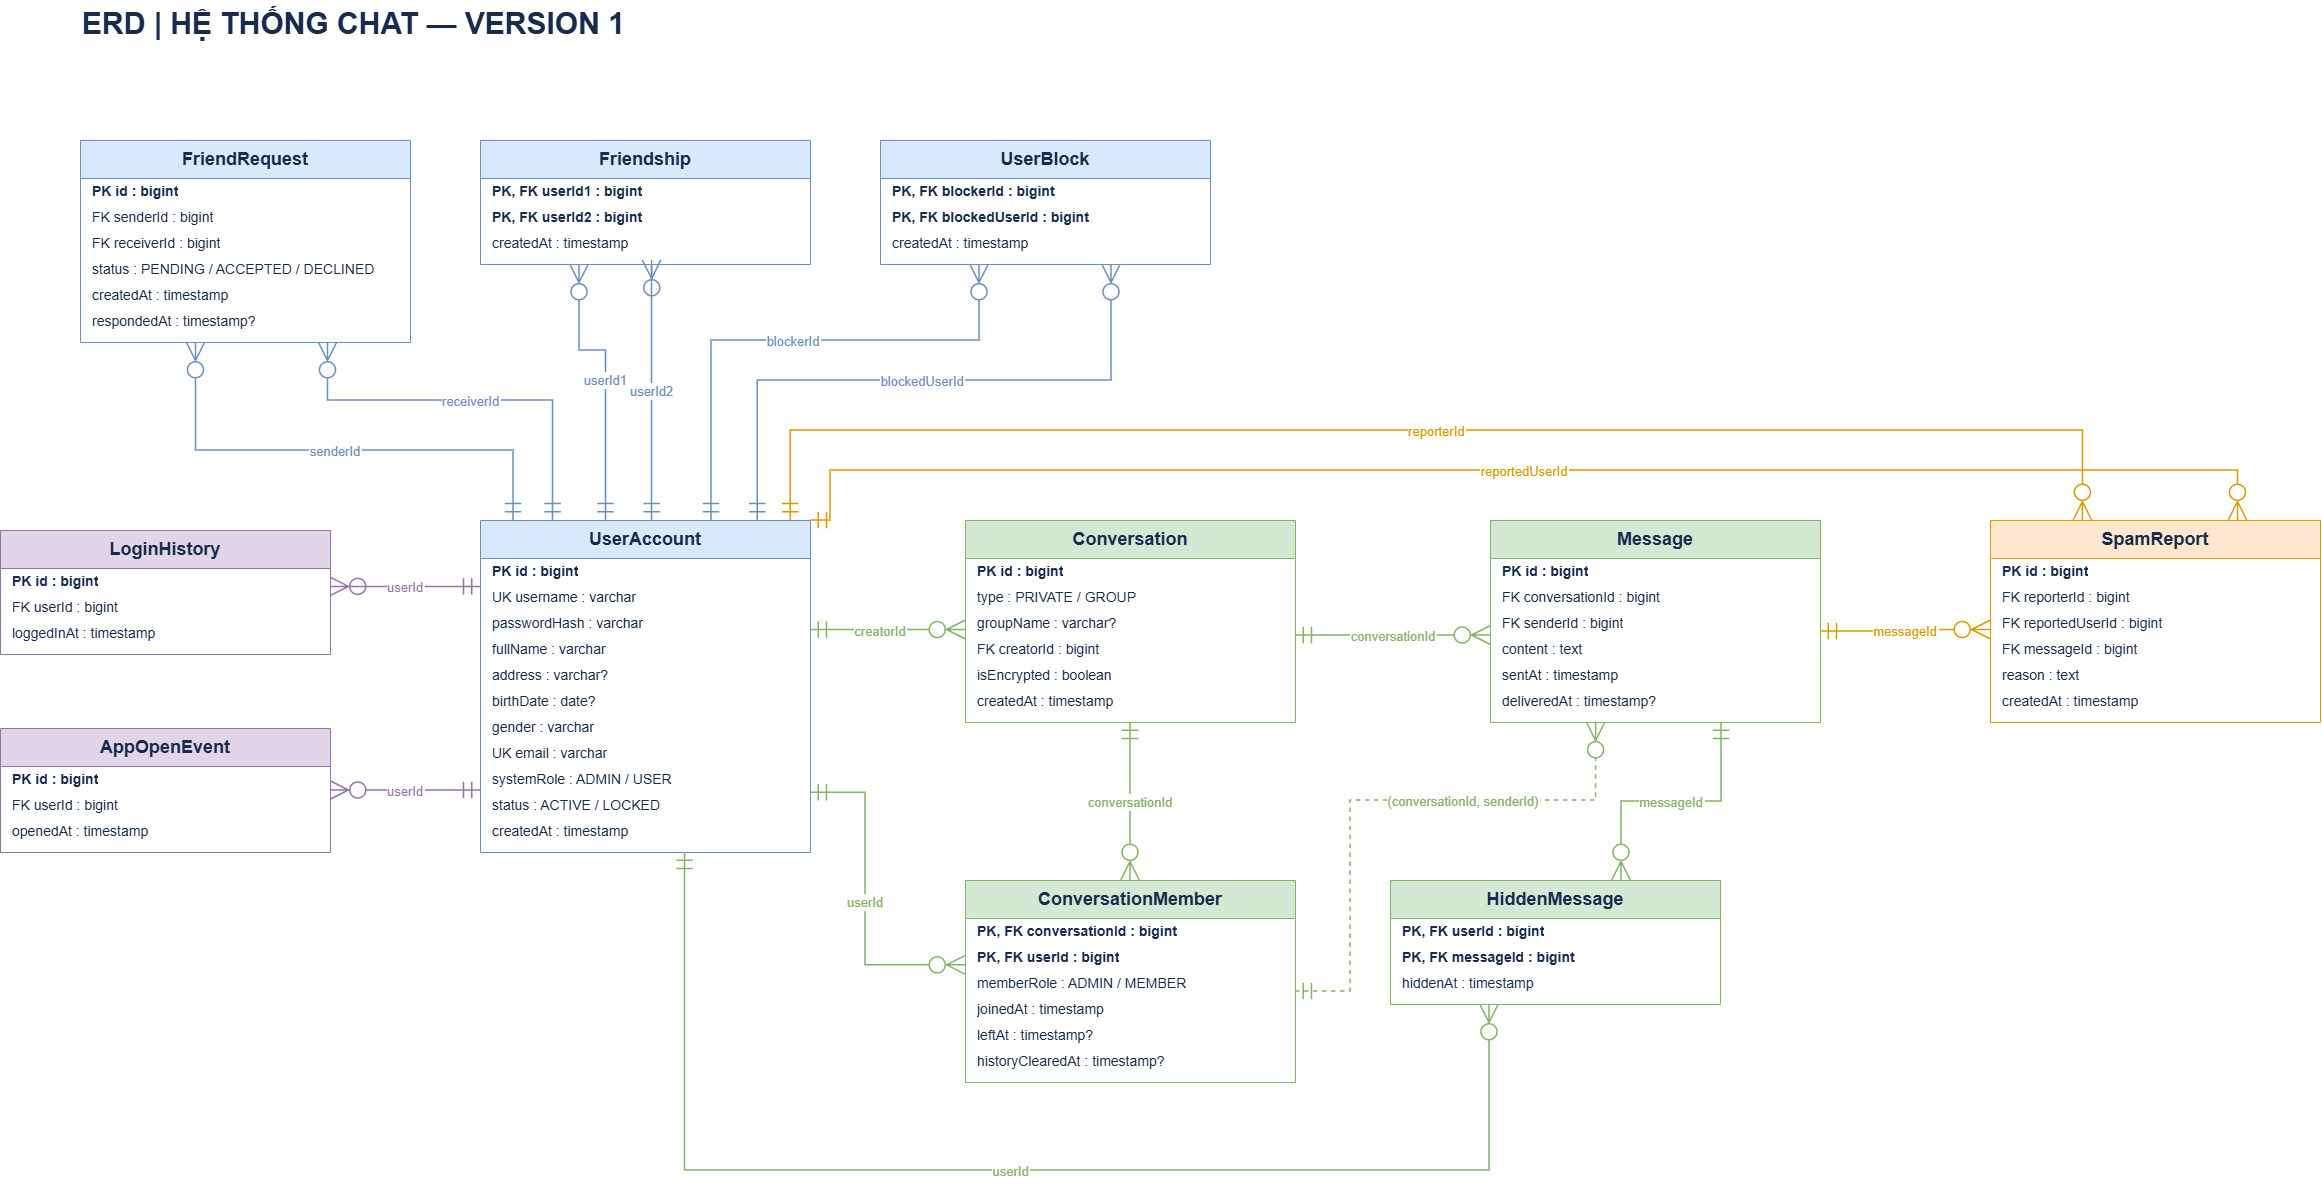
\includegraphics[width=\linewidth,height=0.83\textheight,keepaspectratio]{images/ERD-chatapp-v1.drawio.png}
  \caption{Entity relationship diagram of the chat system.}
  \label{fig:erd-chatapp-v1}
\end{figure}
\end{landscape}

Entity and attribute names in the text match the diagram. Data types in the ERD
are logical; string lengths, default values and the on-delete policy are decided
when the PostgreSQL script is finished.

\paragraph{Data dictionary}
\mbox{}\par

The table below describes the attributes of the 11 entities in the ERD. For a
composite primary key, the attributes marked PK in the same entity form one key
together; each attribute on its own does not have to be unique. Attributes without
a question mark in the figure are expected to have a value; fields that may be
empty are noted in the key and nullability column.

\begingroup
\small
\setlength{\tabcolsep}{4pt}
\begin{longtable}{|L{3.6cm}|L{1.8cm}|L{2.9cm}|L{\dimexpr\textwidth-8.3cm-8\tabcolsep-5\arrayrulewidth\relax}|}
  \caption{Entities and attributes of the database design}
  \label{tab:data-dictionary}\\
  \hline
  \textbf{Attribute} & \textbf{Logical type} & \textbf{Key and nullability} & \textbf{Meaning}\\
  \hline
  \endfirsthead
  \hline
  \textbf{Attribute} & \textbf{Logical type} & \textbf{Key and nullability} & \textbf{Meaning}\\
  \hline
  \endhead
  \multicolumn{4}{|l|}{\textbf{UserAccount}}\\*
  \hline
  \texttt{id} & \texttt{bigint} & PK; Required & Account identifier.\\
  \hline
  \texttt{username} & \texttt{varchar} & UK; Required & Unique username; the upper/lower case rule is decided when the database is created.\\
  \hline
  \texttt{passwordHash} & \texttt{varchar} & Required & Password hash; passwords are never stored as plain text.\\
  \hline
  \texttt{fullName} & \texttt{varchar} & Required & The user's full name.\\
  \hline
  \texttt{address} & \texttt{varchar} & Nullable & Address in the personal profile.\\
  \hline
  \texttt{birthDate} & \texttt{date} & Nullable & Date of birth, separate from activity timestamps.\\
  \hline
  \texttt{gender} & \texttt{varchar} & Required & Gender in the personal profile.\\
  \hline
  \texttt{email} & \texttt{varchar} & UK; Required & Unique email, used for contact and password reset.\\
  \hline
  \texttt{systemRole} & \texttt{varchar} & Required & System role: \texttt{ADMIN} or \texttt{USER}.\\
  \hline
  \texttt{status} & \texttt{varchar} & Required & Account status: \texttt{ACTIVE} or \texttt{LOCKED}.\\
  \hline
  \texttt{createdAt} & \texttt{timestamp} & Required & When the account was created; used for new-registration statistics.\\
  \hline
  \multicolumn{4}{|l|}{\textbf{FriendRequest}}\\*
  \hline
  \texttt{id} & \texttt{bigint} & PK; Required & Friend request identifier.\\
  \hline
  \texttt{senderId} & \texttt{bigint} & FK; Required & Account that sent the request, references \texttt{UserAccount.id}.\\
  \hline
  \texttt{receiverId} & \texttt{bigint} & FK; Required & Account that received the request, references \texttt{UserAccount.id}.\\
  \hline
  \texttt{status} & \texttt{varchar} & Required & Status \texttt{PENDING}, \texttt{ACCEPTED} or \texttt{DECLINED}.\\
  \hline
  \texttt{createdAt} & \texttt{timestamp} & Required & When the request was sent.\\
  \hline
  \texttt{respondedAt} & \texttt{timestamp} & Nullable & When it was accepted or declined; empty while pending.\\
  \hline
  \multicolumn{4}{|l|}{\textbf{Friendship}}\\*
  \hline
  \texttt{userId1} & \texttt{bigint} & Composite PK, FK; Required & First account; references \texttt{UserAccount.id}.\\
  \hline
  \texttt{userId2} & \texttt{bigint} & Composite PK, FK; Required & Second account; references \texttt{UserAccount.id}.\\
  \hline
  \texttt{createdAt} & \texttt{timestamp} & Required & When the friendship started.\\
  \hline
  \multicolumn{4}{|l|}{\textbf{UserBlock}}\\*
  \hline
  \texttt{blockerId} & \texttt{bigint} & Composite PK, FK; Required & Account that blocks, references \texttt{UserAccount.id}.\\
  \hline
  \texttt{blockedUserId} & \texttt{bigint} & Composite PK, FK; Required & Account that is blocked, references \texttt{UserAccount.id}.\\
  \hline
  \texttt{createdAt} & \texttt{timestamp} & Required & When the block was created.\\
  \hline
  \multicolumn{4}{|l|}{\textbf{Conversation}}\\*
  \hline
  \texttt{id} & \texttt{bigint} & PK; Required & Conversation identifier.\\
  \hline
  \texttt{type} & \texttt{varchar} & Required & Conversation type: \texttt{PRIVATE} or \texttt{GROUP}.\\
  \hline
  \texttt{groupName} & \texttt{varchar} & Nullable & Group name; not used for private conversations.\\
  \hline
  \texttt{creatorId} & \texttt{bigint} & FK; Required & Account that created the conversation, references \texttt{UserAccount.id}.\\
  \hline
  \texttt{isEncrypted} & \texttt{boolean} & Required & Flag for an encrypted group; it does not replace key management data.\\
  \hline
  \texttt{createdAt} & \texttt{timestamp} & Required & When the conversation or group was created.\\
  \hline
  \multicolumn{4}{|l|}{\textbf{ConversationMember}}\\*
  \hline
  \texttt{conversationId} & \texttt{bigint} & Composite PK, FK; Required & Conversation joined, references \texttt{Conversation.id}.\\
  \hline
  \texttt{userId} & \texttt{bigint} & Composite PK, FK; Required & Participant, references \texttt{UserAccount.id}.\\
  \hline
  \texttt{memberRole} & \texttt{varchar} & Required & Role in the conversation: \texttt{ADMIN} or \texttt{MEMBER}; separate from the system role.\\
  \hline
  \texttt{joinedAt} & \texttt{timestamp} & Required & When the member joined the conversation.\\
  \hline
  \texttt{leftAt} & \texttt{timestamp} & Nullable & When the member left or was removed from the group; empty while still a member.\\
  \hline
  \texttt{historyClearedAt} & \texttt{timestamp} & Nullable & Point before which the whole history is hidden for this member, since clearing history affects only that person.\\
  \hline
  \multicolumn{4}{|l|}{\textbf{Message}}\\*
  \hline
  \texttt{id} & \texttt{bigint} & PK; Required & Message identifier.\\
  \hline
  \texttt{conversationId} & \texttt{bigint} & FK; Required & Conversation of the message, references \texttt{Conversation.id}; also part of the sender's composite foreign key.\\
  \hline
  \texttt{senderId} & \texttt{bigint} & FK; Required & Sender; with \texttt{conversationId} it references the key of \texttt{ConversationMember}.\\
  \hline
  \texttt{content} & \texttt{text} & Required & Message content. How encrypted content is stored still needs to be designed.\\
  \hline
  \texttt{sentAt} & \texttt{timestamp} & Required & When the message was sent; used to order the history and filter by time.\\
  \hline
  \texttt{deliveredAt} & \texttt{timestamp} & Nullable & When a private message reached its recipient: equal to
  \texttt{sentAt} if the recipient was online, or the time they next signed in if it had to wait; empty while waiting
  and for group messages.\\
  \hline
  \multicolumn{4}{|l|}{\textbf{HiddenMessage}}\\*
  \hline
  \texttt{userId} & \texttt{bigint} & Composite PK, FK; Required & User who hid the message, references \texttt{UserAccount.id}.\\
  \hline
  \texttt{messageId} & \texttt{bigint} & Composite PK, FK; Required & Hidden message, references \texttt{Message.id}.\\
  \hline
  \texttt{hiddenAt} & \texttt{timestamp} & Required & When the user hid the message from their history.\\
  \hline
  \multicolumn{4}{|l|}{\textbf{SpamReport}}\\*
  \hline
  \texttt{id} & \texttt{bigint} & PK; Required & Spam report identifier.\\
  \hline
  \texttt{reporterId} & \texttt{bigint} & FK; Required & Reporting account, references \texttt{UserAccount.id}.\\
  \hline
  \texttt{reportedUserId} & \texttt{bigint} & FK; Required & Reported account, references \texttt{UserAccount.id}.\\
  \hline
  \texttt{messageId} & \texttt{bigint} & FK; Required & Related message, references \texttt{Message.id}.\\
  \hline
  \texttt{reason} & \texttt{text} & Required & Reason or description of the report.\\
  \hline
  \texttt{createdAt} & \texttt{timestamp} & Required & When the report was sent; used for filtering and sorting.\\
  \hline
  \multicolumn{4}{|l|}{\textbf{LoginHistory}}\\*
  \hline
  \texttt{id} & \texttt{bigint} & PK; Required & Sign-in identifier.\\
  \hline
  \texttt{userId} & \texttt{bigint} & FK; Required & Account that signed in, references \texttt{UserAccount.id}.\\
  \hline
  \texttt{loggedInAt} & \texttt{timestamp} & Required & Time of the successful sign-in.\\
  \hline
  \multicolumn{4}{|l|}{\textbf{AppOpenEvent}}\\*
  \hline
  \texttt{id} & \texttt{bigint} & PK; Required & App-open identifier.\\
  \hline
  \texttt{userId} & \texttt{bigint} & FK; Required & Account whose activity is recorded, references \texttt{UserAccount.id}.\\
  \hline
  \texttt{openedAt} & \texttt{timestamp} & Required & When the app was opened; used for app-open and active-user statistics.\\
  \hline
\end{longtable}
\endgroup

Timestamps used for sorting and statistics must be stored and interpreted in one
consistent time zone when the script and the JDBC connection are created. Usernames,
emails, account status and request status also need consistent value conventions.

\paragraph{Main relationships}
\mbox{}\par

An account can send or receive many friend requests, appear in many friendships
and blocks, and take part in many conversations. Where a relationship has two
roles, two attributes reference \texttt{UserAccount.id} with different meanings,
for example the sender and the receiver of a friend request.

\begin{itemize}
  \item \textbf{Accounts and friendships:}
    \texttt{FriendRequest.senderId} and \texttt{receiverId},
    the two attributes of the \texttt{Friendship} primary key,
    and \texttt{UserBlock.blockerId} and \texttt{blockedUserId}
    all reference the matching account.
  \item \textbf{Accounts and conversations:}
    \texttt{Conversation.creatorId} references the creator.
    The many-to-many relationship between accounts and conversations is
    resolved through \texttt{ConversationMember}, whose composite primary key is
    \texttt{(conversationId, userId)}.
  \item \textbf{Conversations and messages:}
    every message belongs to one conversation. The pair
    \texttt{(conversationId, senderId)} in \texttt{Message}
    references the primary key of \texttt{ConversationMember}, which ensures
    the sender has a membership record in that conversation.
    Whether the sender is still a member when sending is checked by the backend.
  \item \textbf{Messages and personal history:}
    \texttt{HiddenMessage} links a user to a message.
    The composite primary key \texttt{(userId, messageId)} prevents recording
    the same hidden message twice for that user.
  \item \textbf{Messages and spam reports:}
    \texttt{SpamReport} references the reporter, the reported account
    and the related message; a message can appear in several reports.
  \item \textbf{Accounts and activity:}
    each \texttt{LoginHistory} or \texttt{AppOpenEvent} record
    belongs to one account; an account can have many records over time.
  \item \textbf{Encryption keys:}
    each account has at most one \texttt{UserKey}. A group has many
    \texttt{GroupKey} versions, keyed by \texttt{(conversationId, keyVersion)};
    each version has one \texttt{GroupKeyShare} per member who may read it.
    \texttt{Message.(conversationId, keyVersion)} references the key version
    used to encrypt the message.
  \item \textbf{Group events:}
    a group has many \texttt{GroupEvent} records; \texttt{actorId} and
    \texttt{targetUserId} reference the accounts involved.
  \item \textbf{Account locks:}
    \texttt{AccountLockLog} references the affected account, the acting
    administrator and, optionally, the \texttt{SpamReport} that led to the lock.
\end{itemize}

\paragraph{Planned constraints and data rules}
\mbox{}\par

Primary keys, foreign keys, unique constraints and \texttt{CHECK} constraints are
implemented in \texttt{script/create\_database.sql}; for example, a message's sender
must be a member of its conversation, a key share can only go to a member, and a
spam report must point to a message written by the reported account.
Rules about access rights, membership status or changing several records at once
are also checked by the backend; the keys in the ERD alone are not enough for
the whole business logic.

\begin{enumerate}
  \item \textbf{Accounts:} the username and email are unique;
    passwords are stored only as hashes. \texttt{systemRole} separates
    system Admins from Users; \texttt{status} separates active accounts
    from locked ones.
  \item \textbf{Friends and blocks:} the two people in a relationship must differ.
    \texttt{Friendship} stores the ID pair with the convention
    \texttt{userId1 < userId2}, combined with the composite primary key so both
    directions of the same relationship are never stored. A block is directed:
    A blocking B does not mean B blocks A.
  \item \textbf{Conversations and members:} \texttt{type} is
    \texttt{PRIVATE} or \texttt{GROUP}; the group name is used for group conversations.
    A private conversation has two participants; creating a group needs the creator
    and at least one other user. The composite primary key of a member prevents
    the same person from appearing twice in a conversation.
  \item \textbf{Group rights:} \texttt{memberRole} is
    \texttt{ADMIN} or \texttt{MEMBER}, independent of system administrator rights.
    Only group admins can remove members, as the assignment requires. On removal the
    backend sets \texttt{leftAt} instead of deleting the \texttt{ConversationMember}
    row, so the composite foreign key of \texttt{Message} stays valid and the person's
    earlier messages remain; when that person is added again, the same row is reused
    and \texttt{leftAt} is cleared.
    When a message is sent, the backend checks the current membership and rights.
  \item \textbf{Locked accounts:} when \texttt{UserAccount.status} is \texttt{LOCKED},
    nobody can message the account privately, send it or accept its friend requests,
    block it, add it to a group or make it a group admin; others can only unfriend it,
    decline its friend requests and, as group admins, remove it from a group.
  \item \textbf{Message status:} the \textbf{Sent}, \textbf{Waiting} and
    \textbf{Delivered} status of a private message is derived from
    \texttt{Message.deliveredAt}, with no extra status column; group messages only
    show \textbf{Sent}.
  \item \textbf{Spam reports:} the reporter must be allowed to see the related
    content; the reported message must belong to the reported account.
    The backend checks these conditions on top of the foreign keys.
  \item \textbf{Encryption and logs:} a key share can only go to someone with a
    membership record in the group, and a message can only name a key version of
    its own conversation (foreign keys); the backend also ensures that keys exist
    only for group conversations, that \texttt{Message.keyVersion} stays empty in
    private conversations and that a new key version is shared only with current
    members. \texttt{AccountLockLog.action} is \texttt{LOCK} or \texttt{UNLOCK},
    \texttt{GroupEvent.type} takes only the listed values, and a user can report
    the same message only once (check and unique constraints).
  \item \textbf{Consistency:} accepting a friend request updates the request and
    creates the friendship in the same transaction. Blocking and unfriending also
    apply their related changes together to avoid contradictory states.
\end{enumerate}

\paragraph{Clearing history and group encryption}
\mbox{}\par

The proposed design treats clearing history as removing it for the person who does
it. \texttt{HiddenMessage} records each hidden message;
\texttt{ConversationMember.historyClearedAt} marks the point before which the whole
history is cleared for that member. When messages are read, hidden messages and
messages before that point are not shown to that person; other participants keep
their history. The team confirms this interpretation when the design is finalised.

Group encryption follows the end-to-end model of encrypted group chats in
Facebook Messenger~\cite{ref:messenger-e2ee}: the server stores and forwards only ciphertext and never
holds a group key in plain form.

\begin{enumerate}
  \item \textbf{User keys:} at registration the client creates an RSA key pair~\cite{ref:rfc8017}.
    The public key is stored in \texttt{UserKey.publicKey}; the private key is
    encrypted on the client with a key derived from the password (PBKDF2~\cite{ref:rfc8018} with
    \texttt{keySalt}), so the user can sign in from any computer.
  \item \textbf{Turning encryption on:} the client of a group admin creates a
    random AES-256 group key (version 1), wraps it with every member's public key
    and uploads one \texttt{GroupKeyShare} per member;
    \texttt{Conversation.isEncrypted} becomes true.
  \item \textbf{Sending and reading:} the sender encrypts the text with the latest
    key version (AES-GCM~\cite{ref:nist-gcm}, a new IV per message) and stores the version in
    \texttt{Message.keyVersion}; members unwrap the matching share with their
    private key to decrypt.
  \item \textbf{Membership changes:} a new member receives a share of the current
    version. When a member leaves or is removed, an admin's client creates a new
    version and shares it only with the remaining members, so the former member
    cannot read later messages.
  \item \textbf{Turning encryption off:} new messages are stored as plain text with
    an empty \texttt{keyVersion}; earlier messages stay encrypted.
\end{enumerate}

Because the server cannot read encrypted messages, searching them is done on the
client after decryption, the AI assistant is not available in encrypted groups,
and a spam report on an encrypted message carries a plain-text copy in
\texttt{SpamReport.reportedContent} sent by the reporter. Changing a password only
re-encrypts the private key. A password reset (a random password sent by email)
cannot recover the old private key: the user receives a new key pair and can read
older encrypted history again only after a group admin shares the keys with the
new public key.

Deleting an account is a soft delete: the administrator's action sets
\texttt{status} to \texttt{DELETED} and records \texttt{deletedAt}, and no row is
removed. Messages, group history, spam reports and lock history therefore stay
complete, every foreign key to \texttt{UserAccount} rejects physical deletion, and a
deleted account can no longer sign in or be found. Its username and email may be
registered again, because uniqueness only applies to accounts that are not deleted.

\paragraph{Data for statistics}
\mbox{}\par

The model has no separate statistics tables when the figures can be computed from
the source data. The Admin functions map as follows:

\begin{itemize}
  \item \hyperlink{F14}{F14}: reads sign-ins from
    \texttt{LoginHistory}, joins the account profile and sorts by time.
  \item \hyperlink{F17}{F17}--\hyperlink{F18}{F18}: filters
    \texttt{UserAccount.createdAt} by the selected year; counts new accounts
    per month of that year.
  \item \hyperlink{F19}{F19}: counts relationships in \texttt{Friendship};
    \textbf{Total network} is the union of direct friends and friends of friends,
    excluding the account itself and counting each account once.
    \textbf{Friends of friends only} also excludes direct friends; a mutual friend
    is found through two consecutive friendships.
  \item \hyperlink{F20}{F20}: counts app opens from
    \texttt{AppOpenEvent}; checks messages, conversations and members to find
    how many people and groups were chatted with in the selected year.
  \item \hyperlink{F21}{F21}: counts distinct accounts that opened the app in
    each month, not the total number of opens.
\end{itemize}

Sign-in history and app opens are kept apart because reopening the app is not
necessarily a new sign-in. Online/offline status will be determined by the backend
from live connections; an old sign-in record does not prove a user is online.

The \textbf{Period} picker applies one calendar year to tables and charts.
A yearly query covers the start of the year up to the start of the next year in the
system's time zone. Charts always show 12 months; the yearly total of
\textbf{Active users} counts each account once, even when it was active in several
months.

\paragraph{Data for administration extensions}
\mbox{}\par
\texttt{UserAccount.status} holds the current \texttt{ACTIVE}/\texttt{LOCKED}
state, and \texttt{AccountLockLog} keeps its history: each lock or unlock records
the account, the administrator, the time and, when it comes from the spam report
screen, the report. The \textbf{Prior locks} count and the \textbf{Admin lock
history} on the Spam Reports screen read from this table. The backend checks that
\texttt{adminId} belongs to an account with \texttt{systemRole = ADMIN} and
updates the status and the log in one transaction.

The \textbf{Activity} and \textbf{Monitoring} tabs of Chat Groups combine two
sources. Message rows come from \texttt{Message} (an encrypted message is shown
only as ``sent an encrypted message''). Every other change is a
\texttt{GroupEvent} written by the backend in the same transaction as the change
itself: creating the group, renaming it, adding a member, a member leaving or
being removed, a role change, and turning encryption on or off.
\texttt{ConversationMember} alone cannot provide this, because it keeps one row per
member, cannot tell leaving from being removed, and overwrites \texttt{joinedAt}
when a member is added again.


